\documentclass[a4paper]{article}
\usepackage[utf8]{inputenc}
\usepackage{fullpage} % Package to use full page
\usepackage{parskip} % Package to tweak paragraph skipping
\usepackage{tikz} % Package for drawing
\usepackage{listings}
\usepackage{amsmath}
\usepackage{amssymb}
\usepackage{hyperref}
\usepackage{cleveref}
\usepackage{subcaption}

\title{{\small 02427 Advanced Time Series Analysis E18}\\Computer exercise 3}
\author{Niklas Christoffer Petersen}
\date{2018-11-28}

\begin{document}

\maketitle

\section{Part 1}

\subsection{Question 1a}
Plot the realizations of $Y^1$ and $Y^2$ and make a phaseplot of ($Y^1$, $Y^2$).
Repeat for $\sigma = 0.10, 0.20, 0.30$ and $0.40$. Comment on the effect of adding
noise to the equations.

\Cref{fig:part1a-sigma0} shows the realizations of $Y^1$ and $Y^2$ for $\sigma = 0$. We see nice and repeated signal for both after $T \gtrapprox 6$.

\begin{figure}[ht!]
    \centering
    \begin{subfigure}[b]{0.45\textwidth}
        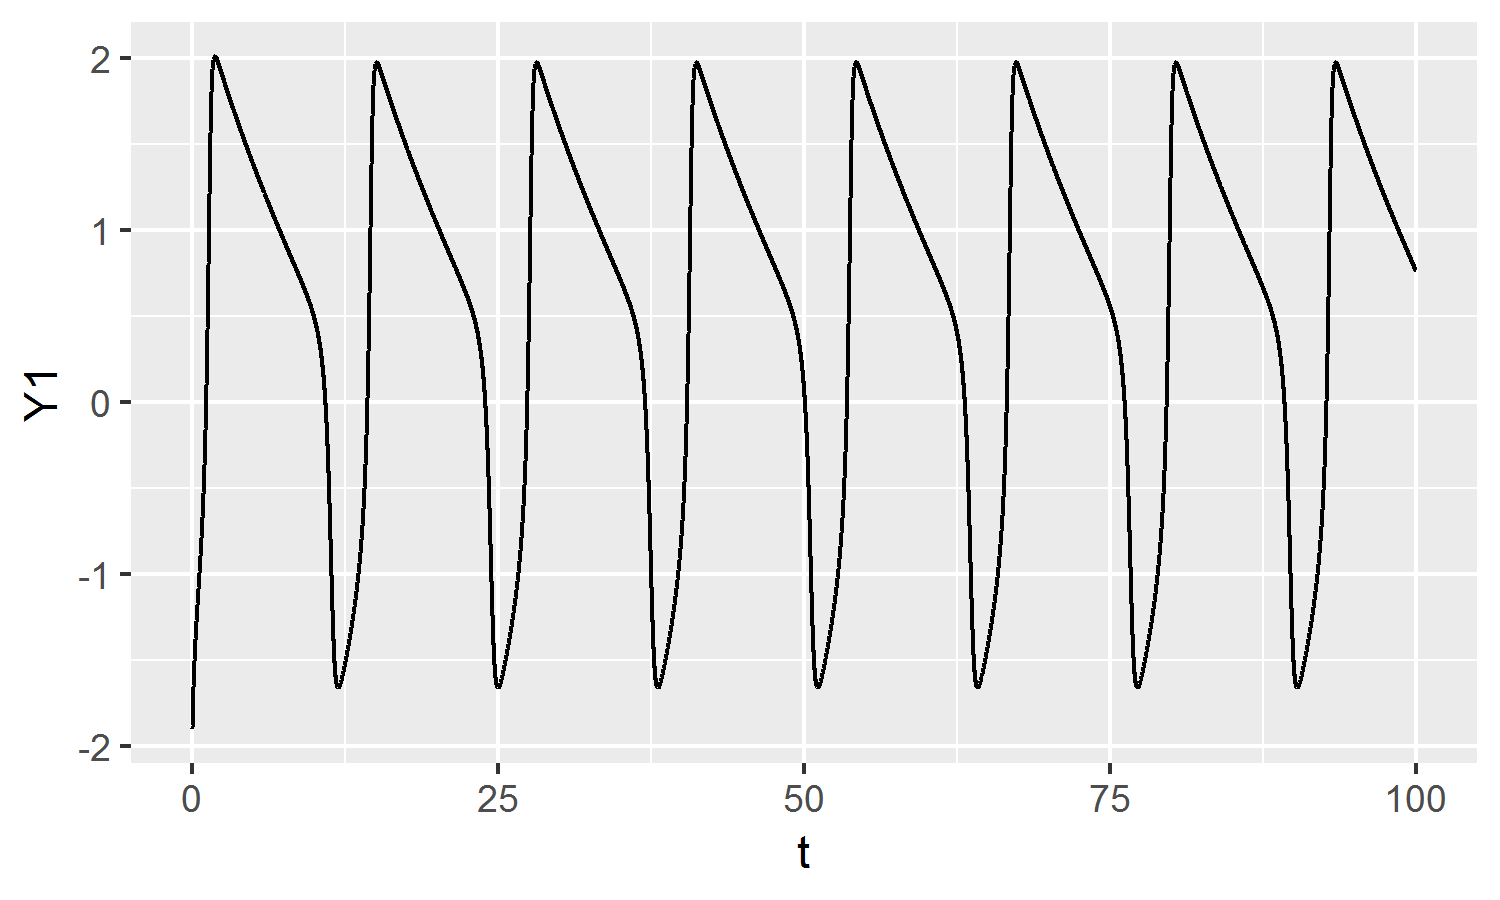
\includegraphics[width=\textwidth]{part1a-sigma0-Y1.png}
        \caption{$Y^1$}
    \end{subfigure}
    ~
    \begin{subfigure}[b]{0.45\textwidth}
        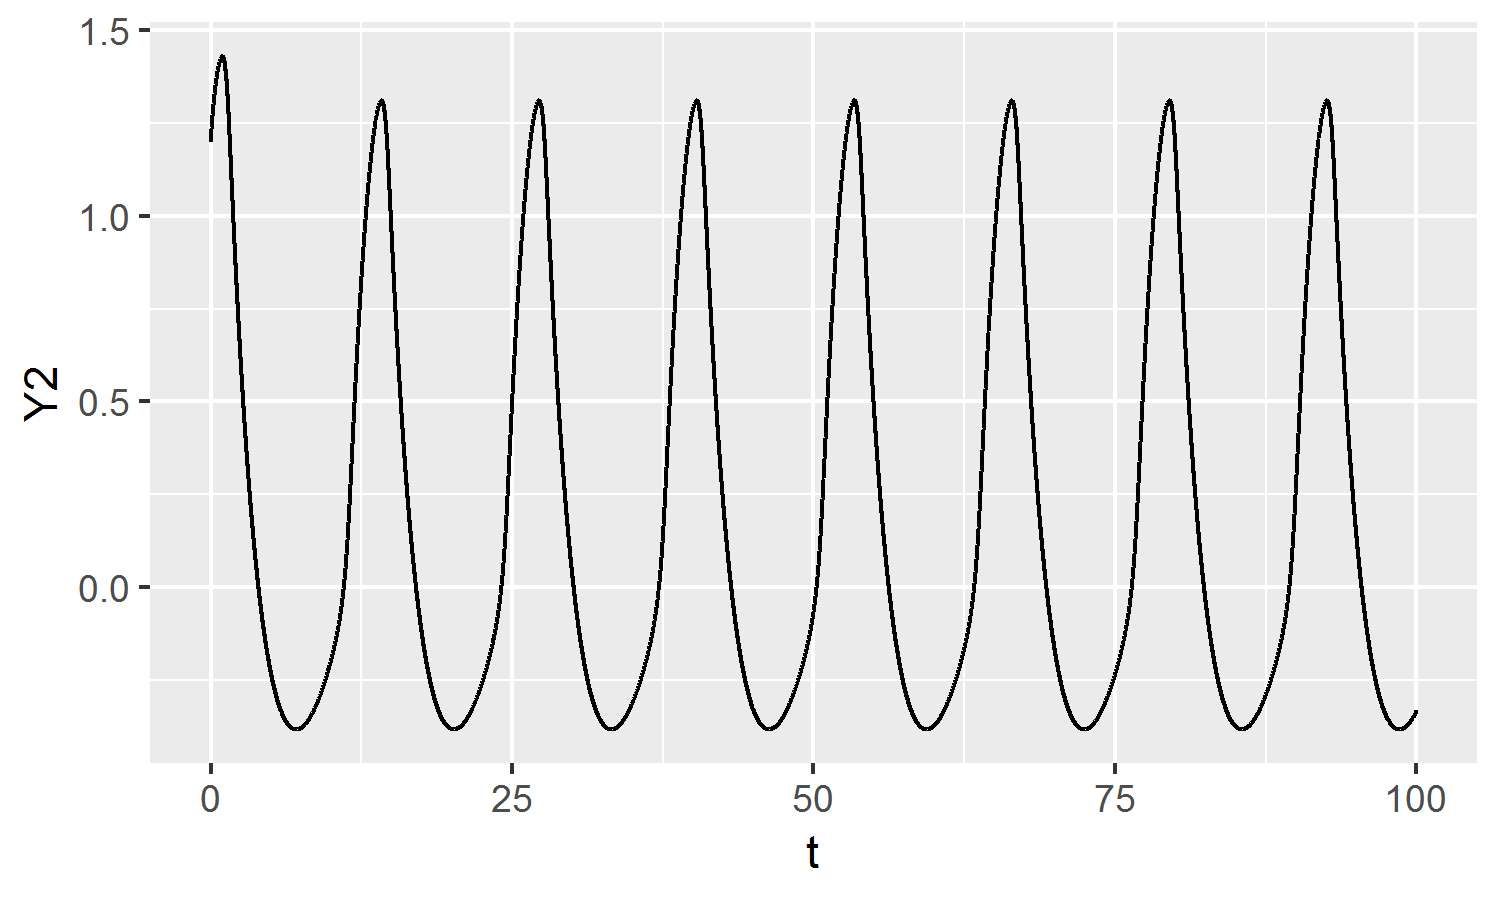
\includegraphics[width=\textwidth]{part1a-sigma0-Y2.png}
        \caption{$Y^2$}
    \end{subfigure}
    \caption{Realized values of $Y^1$ and $Y^2$ for $\sigma = 0$}
    \label{fig:part1a-sigma0}
\end{figure}

\Cref{fig:part1a-sigma0-Y1Y2} shows the phaseplot of ($Y^1$, $Y^2$). Again we see some initial stabilization, but afterward the signal repeats with no variation (as $\sigma = 1$).
\begin{figure}[ht!]
    \centering
    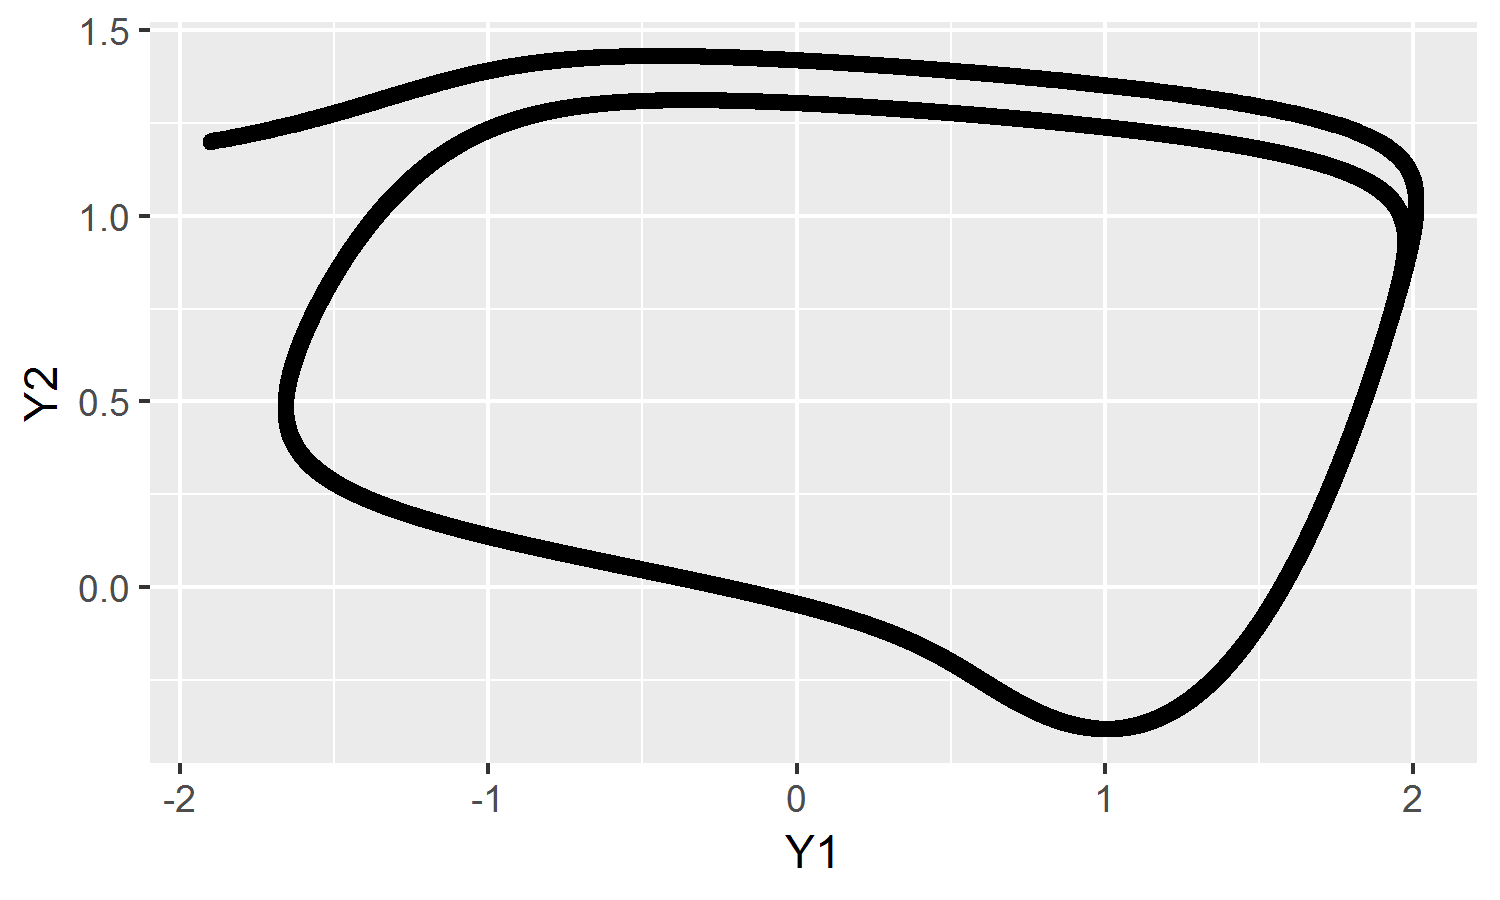
\includegraphics[width=.45\textwidth]{part1a-sigma0-Y1Y2.png}
    \caption{Phase Plot $Y^1$ and $Y^2$ for $\sigma = 0$}
    \label{fig:part1a-sigma0-Y1Y2}
\end{figure}

\clearpage
\begin{figure}
    \centering
    \begin{subfigure}[b]{0.45\textwidth}
        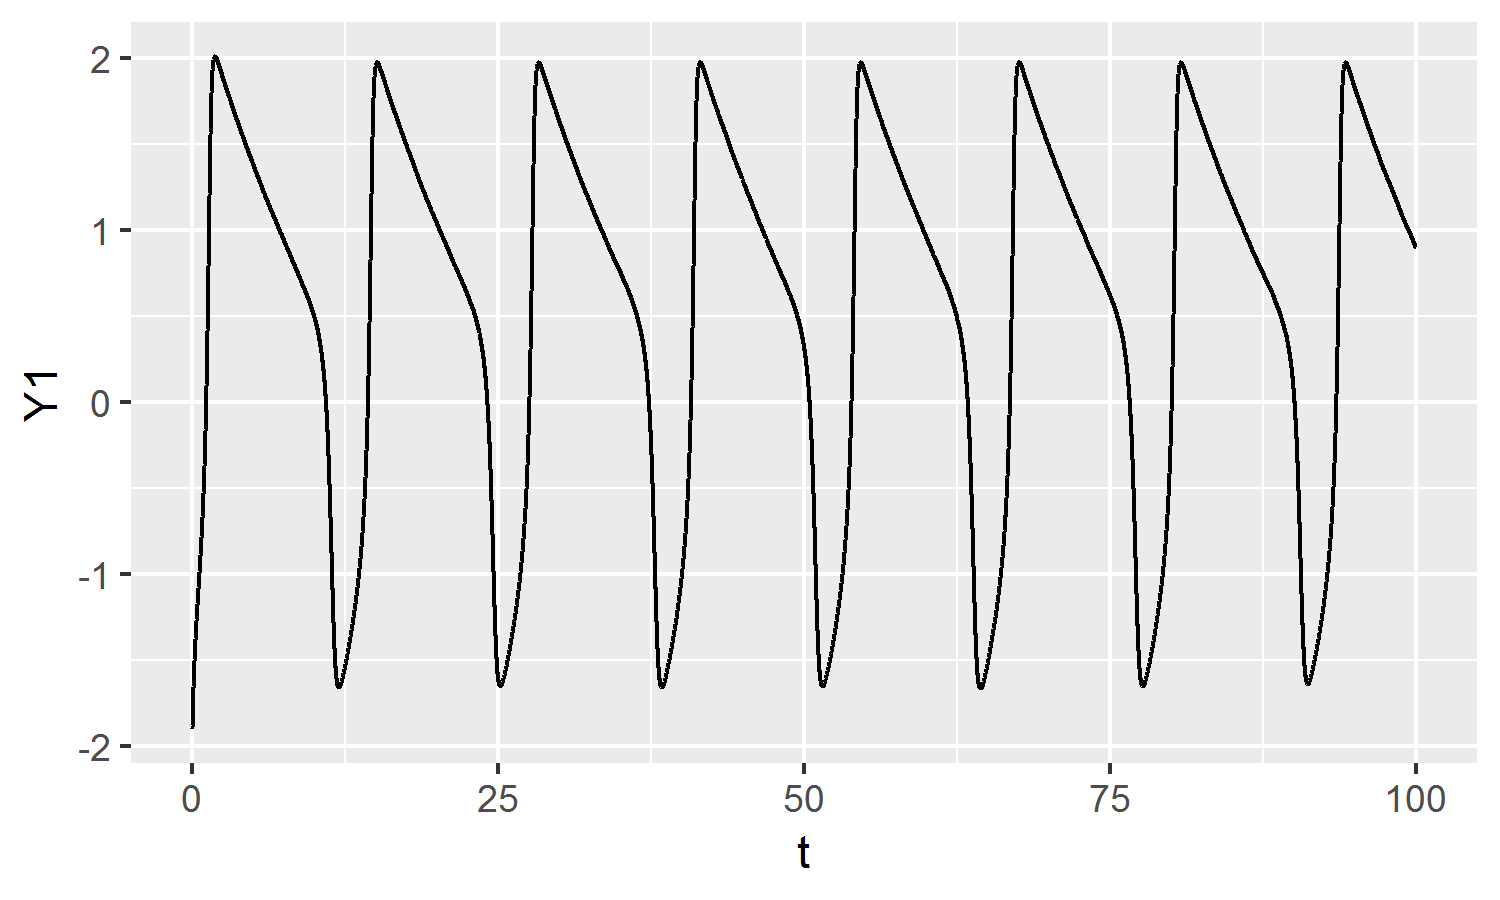
\includegraphics[width=\textwidth]{part1a-sigma1-Y1.png}
        \caption{$Y^1$}
    \end{subfigure}
    ~
    \begin{subfigure}[b]{0.45\textwidth}
        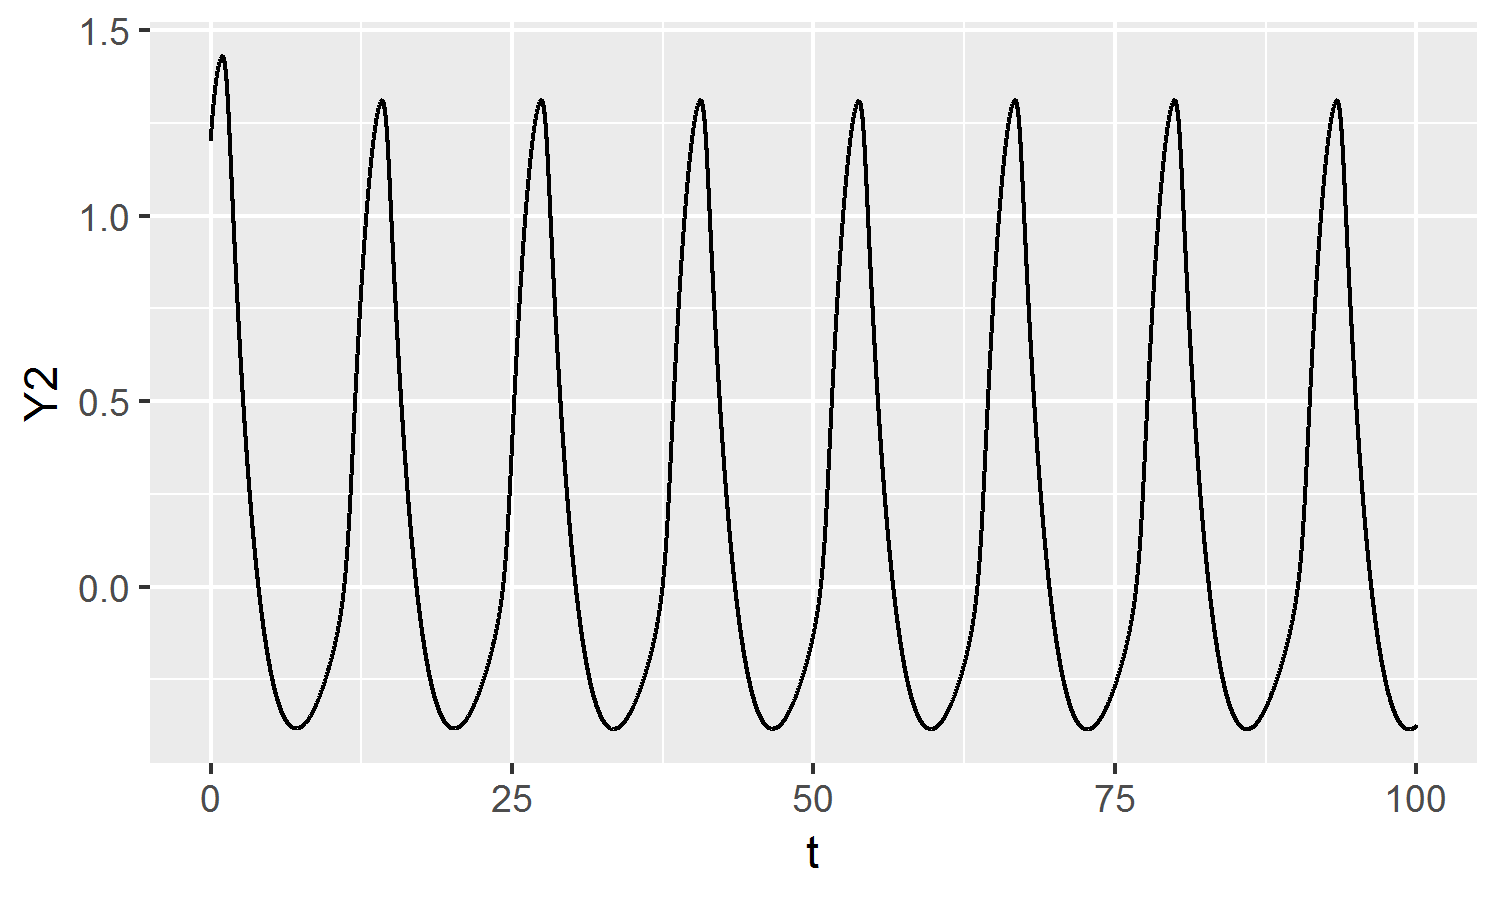
\includegraphics[width=\textwidth]{part1a-sigma1-Y2.png}
        \caption{$Y^2$}
    \end{subfigure}
    \caption{Realized values of $Y^1$ and $Y^2$ for $\sigma = 0.10$}\label{fig:part1a-sigma1}
\end{figure}
\begin{figure}
    \centering
    \begin{subfigure}[b]{0.45\textwidth}
        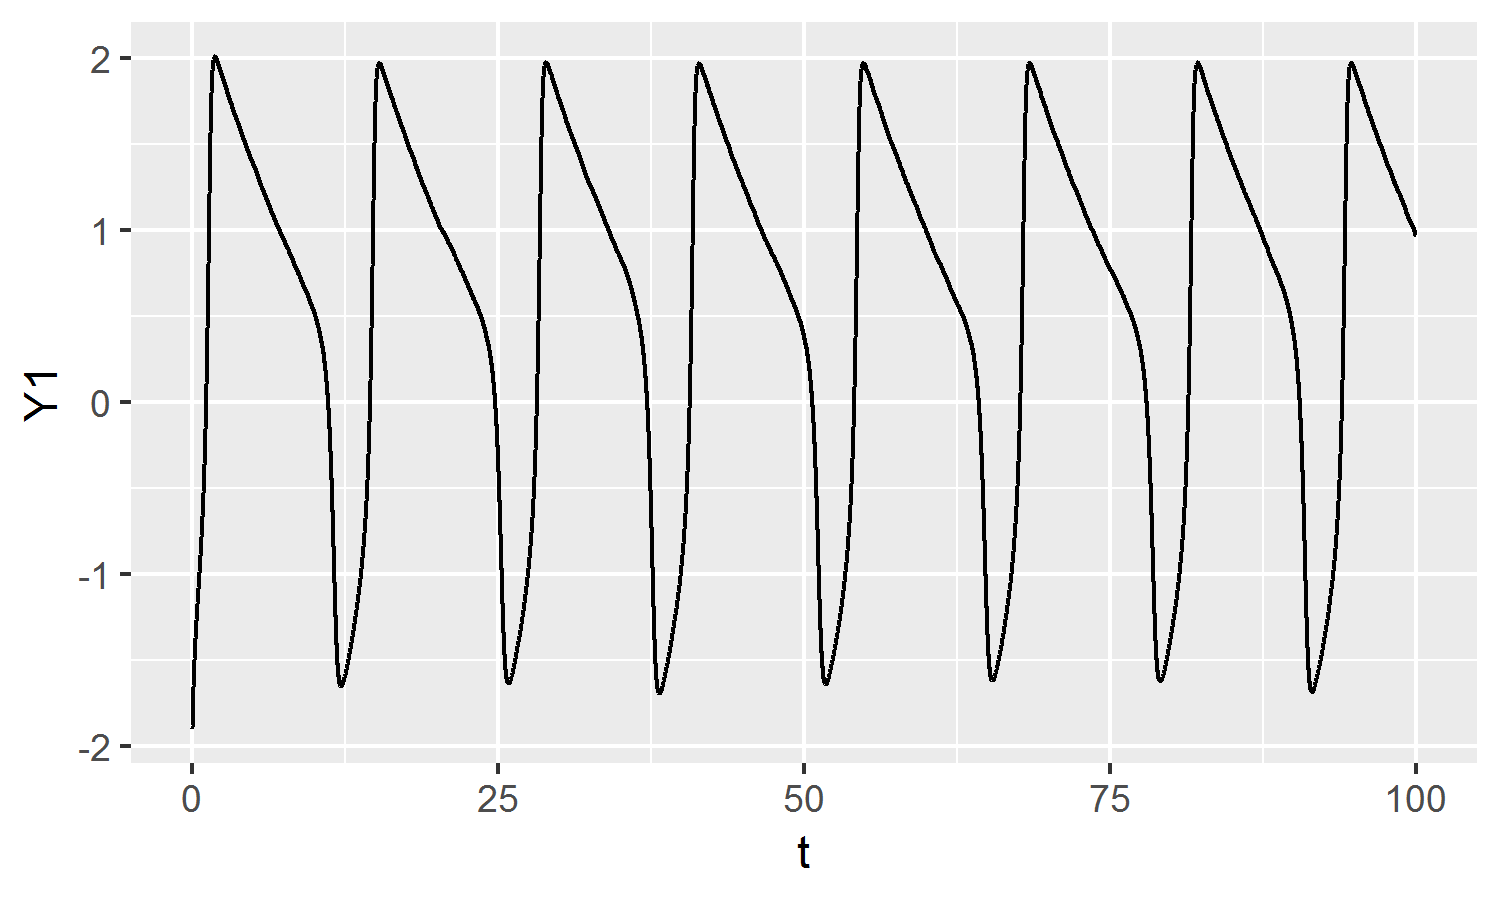
\includegraphics[width=\textwidth]{part1a-sigma2-Y1.png}
        \caption{$Y^1$}
    \end{subfigure}
    ~
    \begin{subfigure}[b]{0.45\textwidth}
        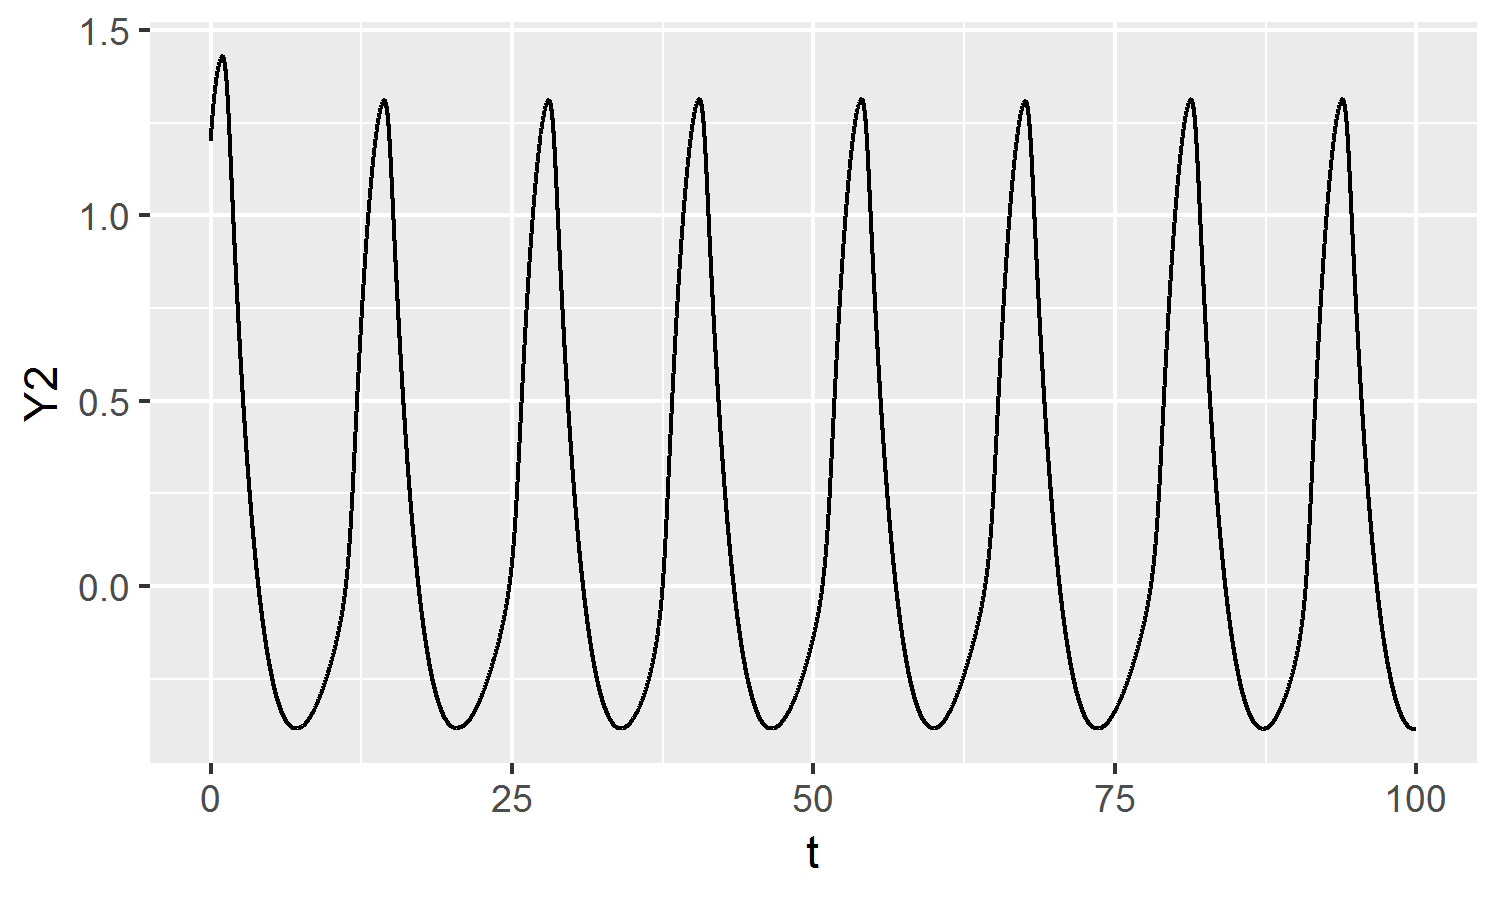
\includegraphics[width=\textwidth]{part1a-sigma2-Y2.png}
        \caption{$Y^2$}
    \end{subfigure}
    \caption{Realized values of $Y^1$ and $Y^2$ for $\sigma = 0.20$}\label{fig:part1a-sigma2}
\end{figure}
\begin{figure}
    \centering
    \begin{subfigure}[b]{0.45\textwidth}
        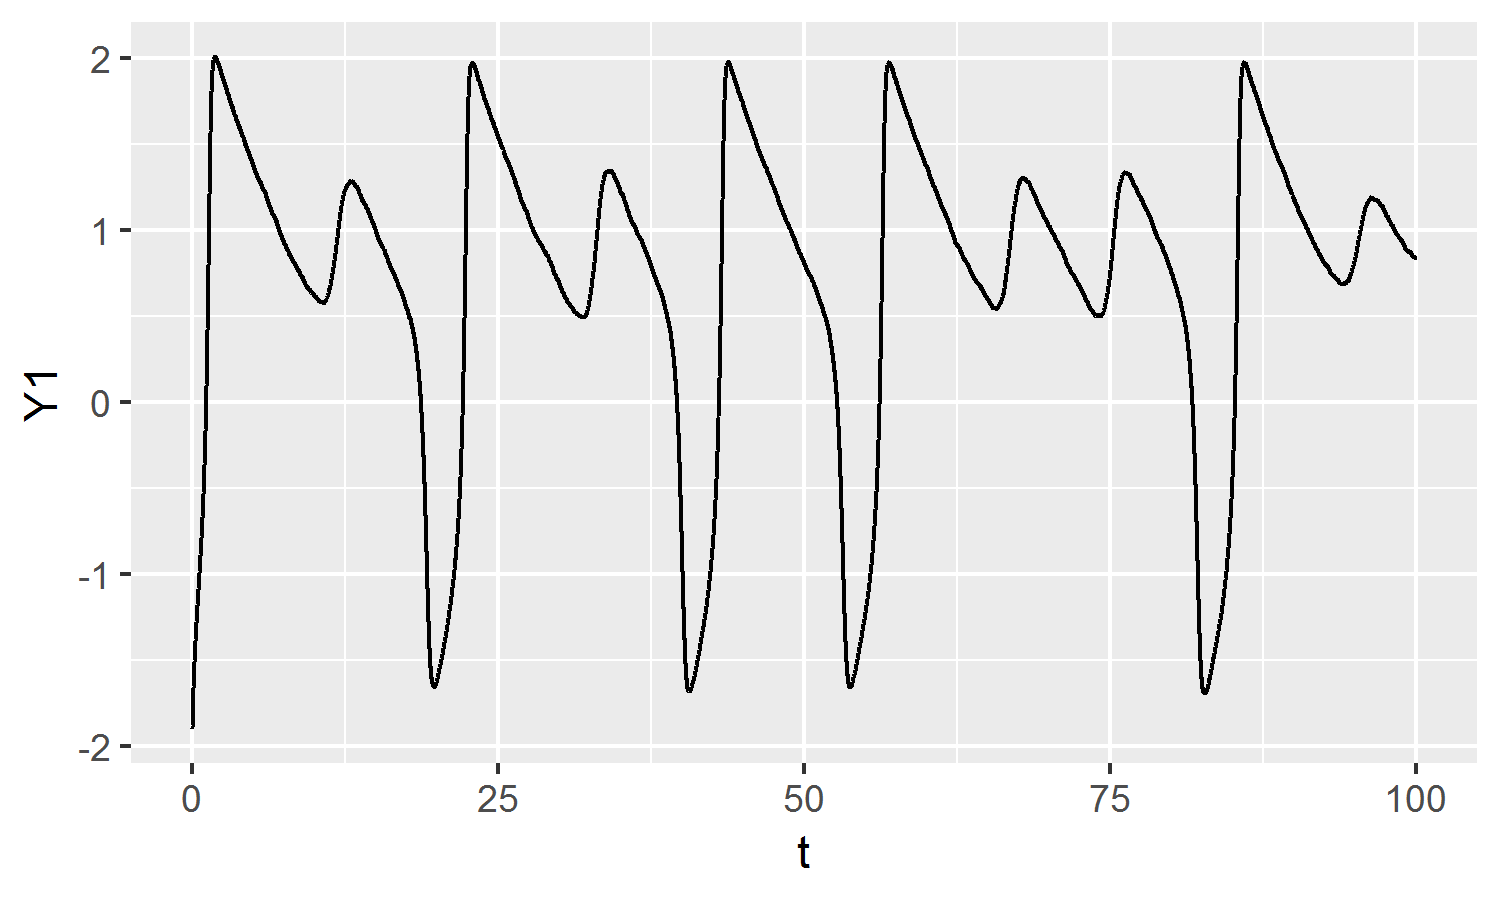
\includegraphics[width=\textwidth]{part1a-sigma3-Y1.png}
        \caption{$Y^1$}
    \end{subfigure}
    ~
    \begin{subfigure}[b]{0.45\textwidth}
        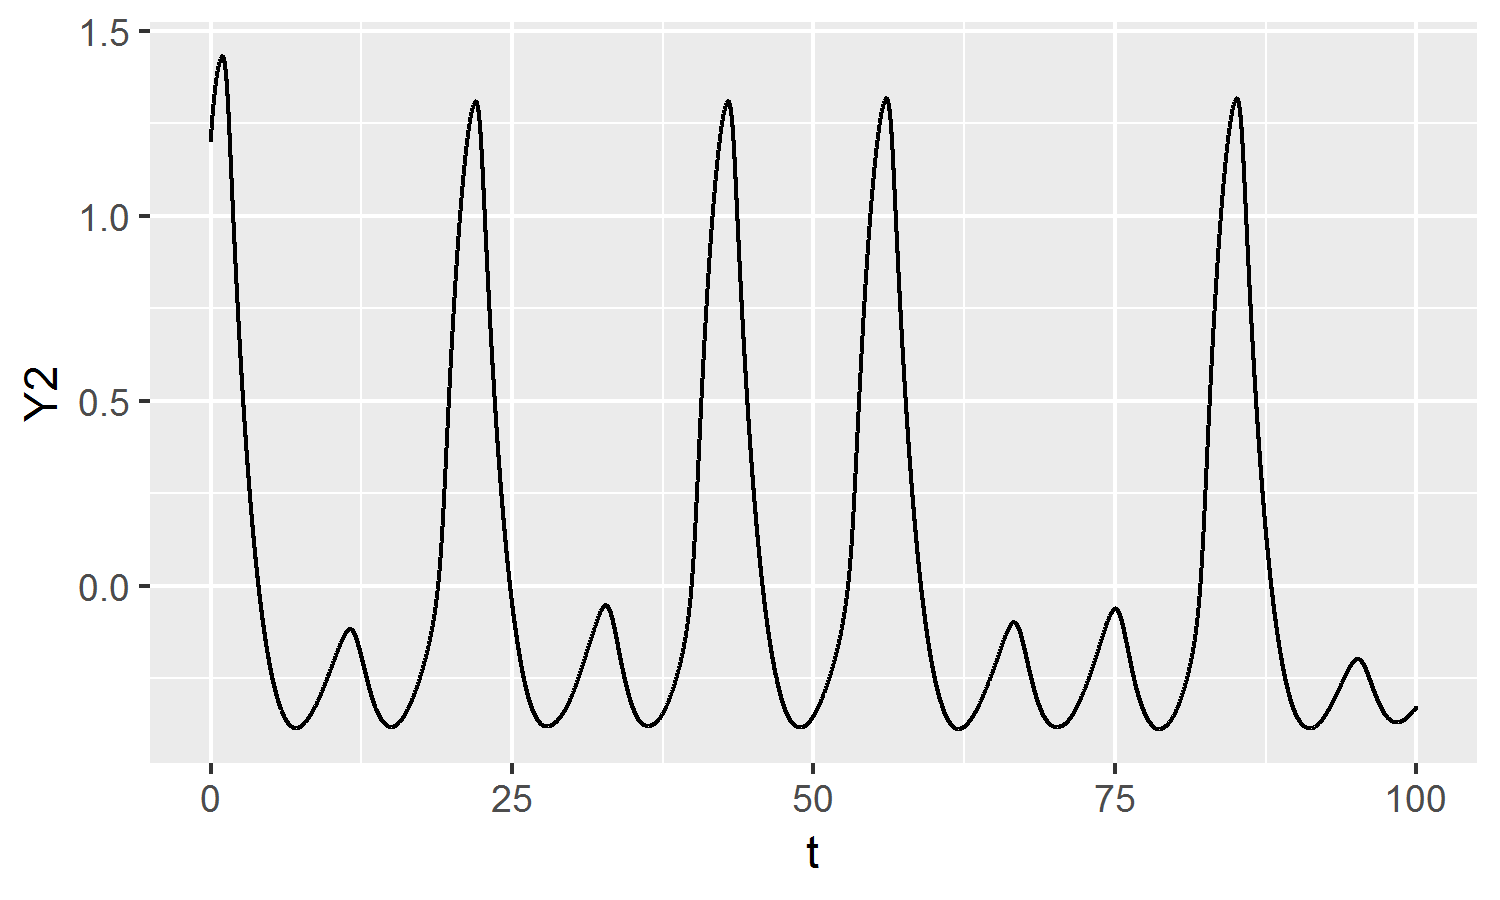
\includegraphics[width=\textwidth]{part1a-sigma3-Y2.png}
        \caption{$Y^2$}
    \end{subfigure}
    \caption{Realized values of $Y^1$ and $Y^2$ for $\sigma = 0.30$}\label{fig:part1a-sigma3}
\end{figure}
\begin{figure}
    \centering
    \begin{subfigure}[b]{0.45\textwidth}
        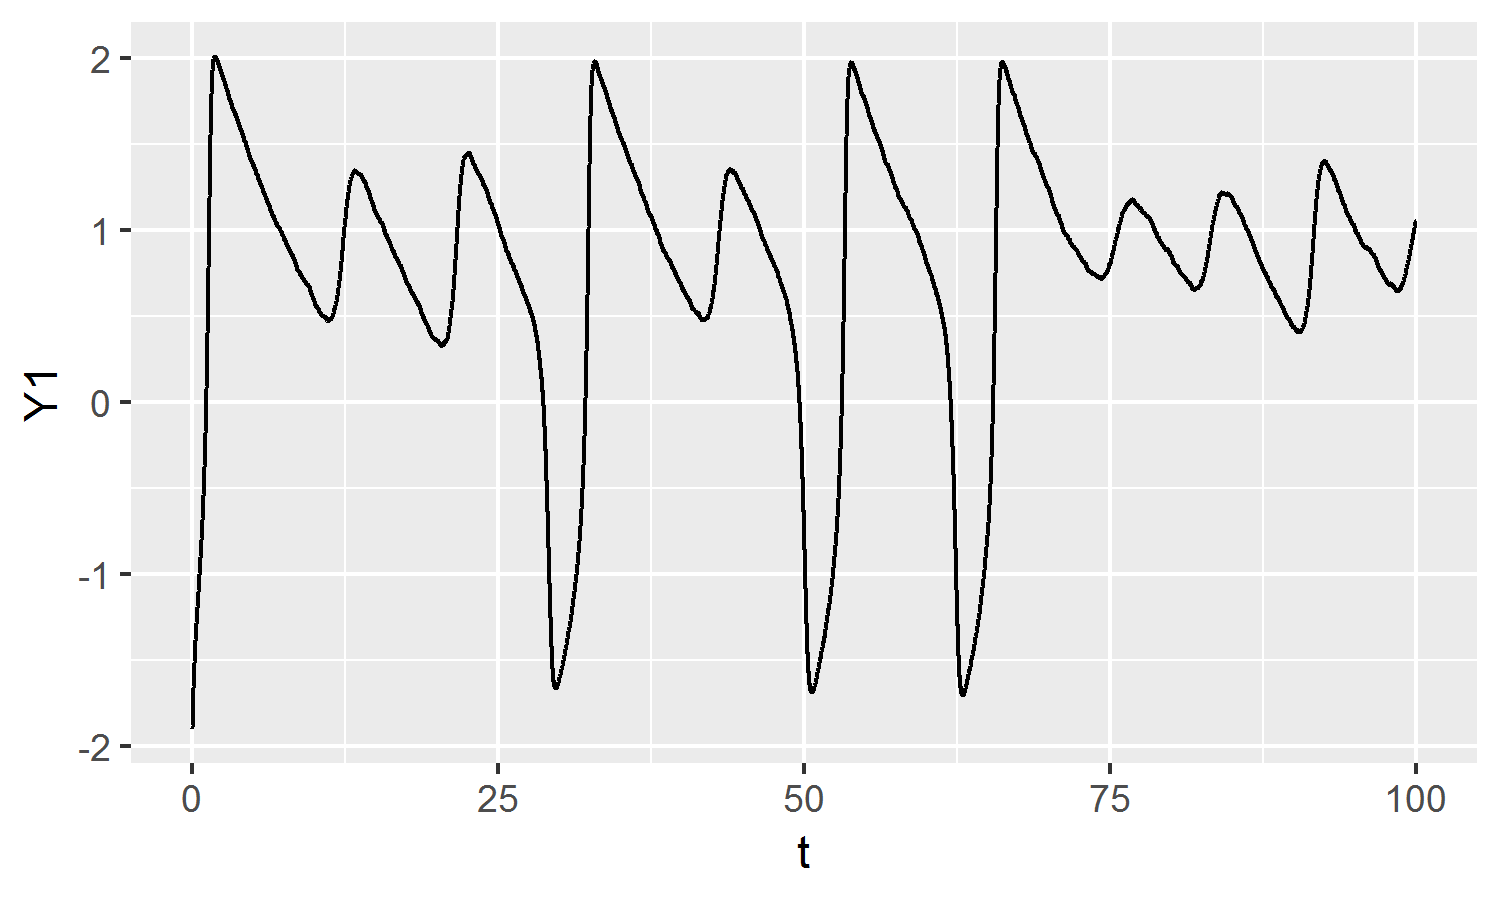
\includegraphics[width=\textwidth]{part1a-sigma4-Y1.png}
        \caption{$Y^1$}
    \end{subfigure}
    ~
    \begin{subfigure}[b]{0.45\textwidth}
        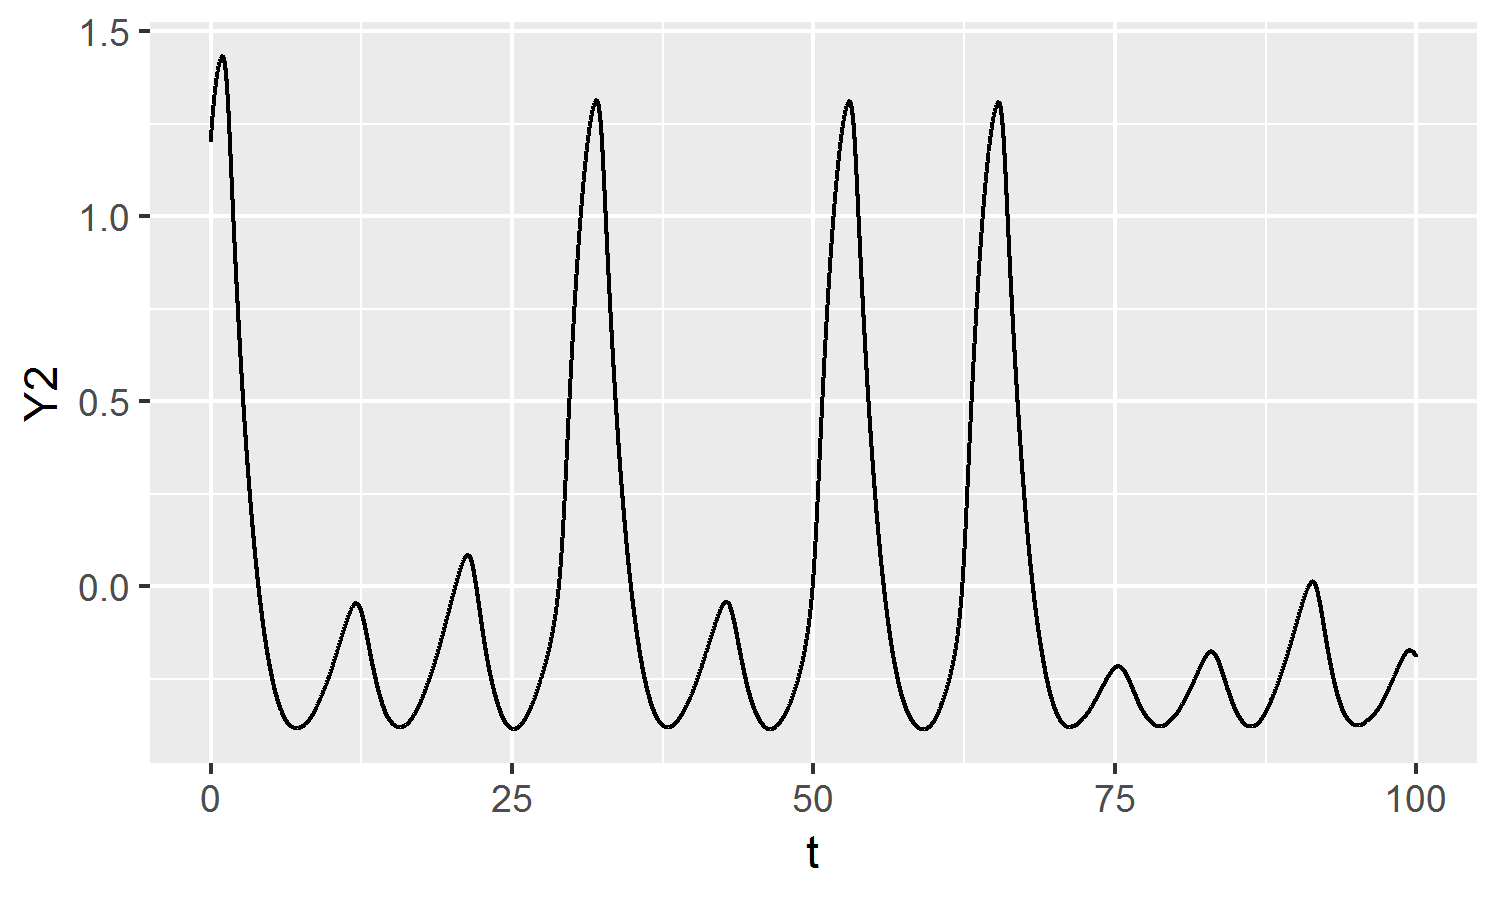
\includegraphics[width=\textwidth]{part1a-sigma4-Y2.png}
        \caption{$Y^2$}
    \end{subfigure}
    \caption{Realized values of $Y^1$ and $Y^2$ for $\sigma = 0.40$}\label{fig:part1a-sigma4}
\end{figure}
\clearpage

We repeat for $\sigma = 0.10, 0.20, 0.30$ and $0.40$ as shown in \Cref{fig:part1a-sigma1,fig:part1a-sigma2,fig:part1a-sigma3,fig:part1a-sigma4}, and phaseplots shown in \Cref{fig:part1a-grid}.

We see that it is still quite stable for $\sigma < 0.20$, but at $\sigma = 0.30$ the system begins to switch between two phases, in a non-obvious way. At $\sigma = 0.40$ the phases become even more chaotic.

\begin{figure}[ht!]
    \centering
    \begin{subfigure}[b]{0.45\textwidth}
        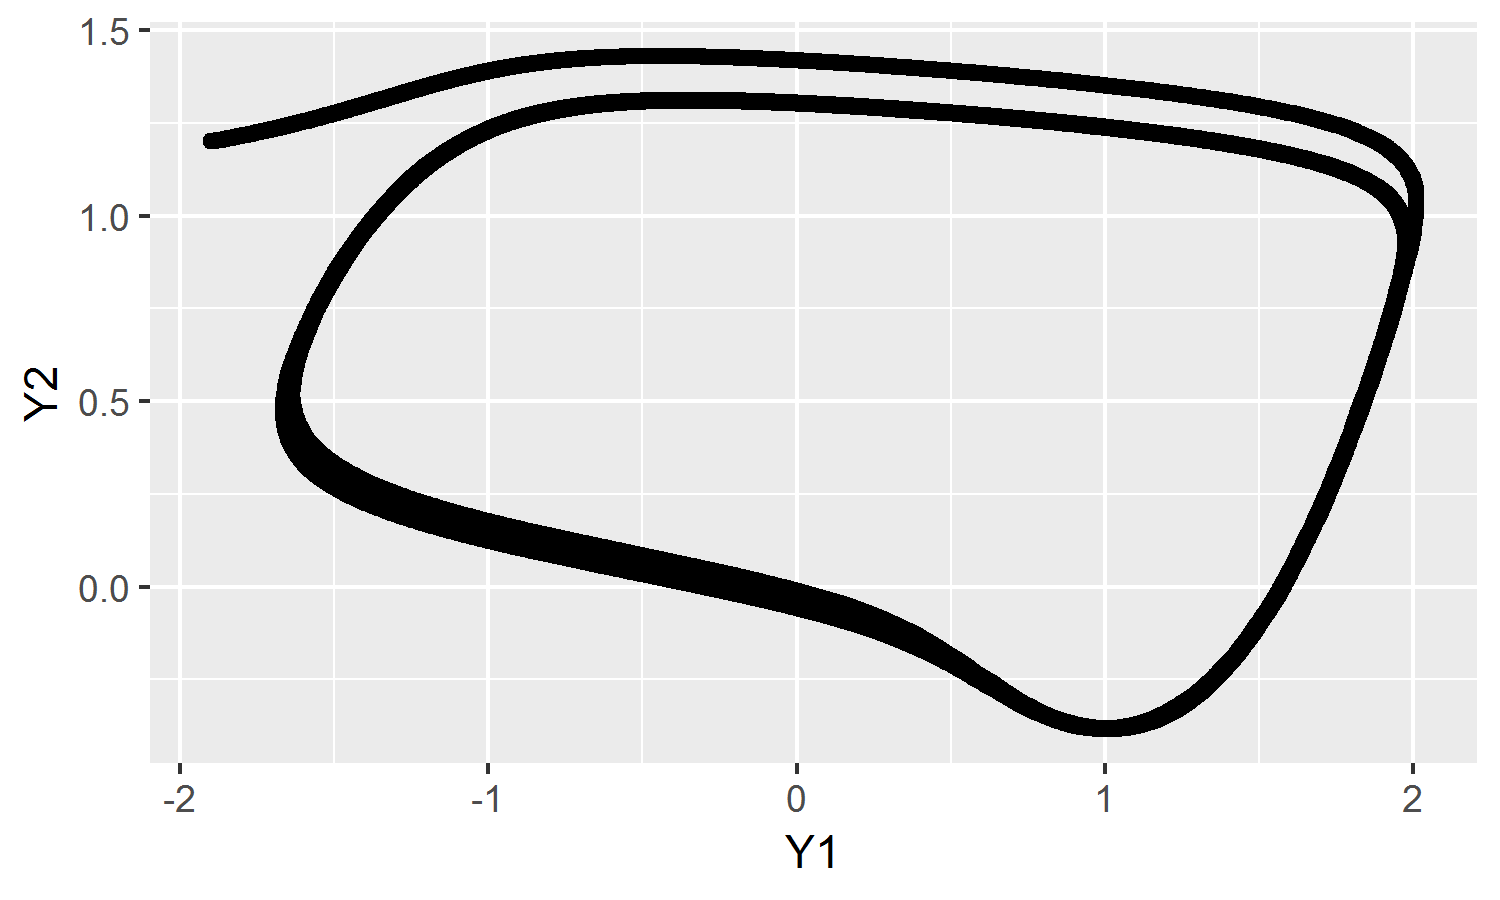
\includegraphics[width=\textwidth]{part1a-sigma1-Y1Y2.png}
        \caption{$\sigma = 0.10$}
    \end{subfigure}
    ~
    \begin{subfigure}[b]{0.45\textwidth}
        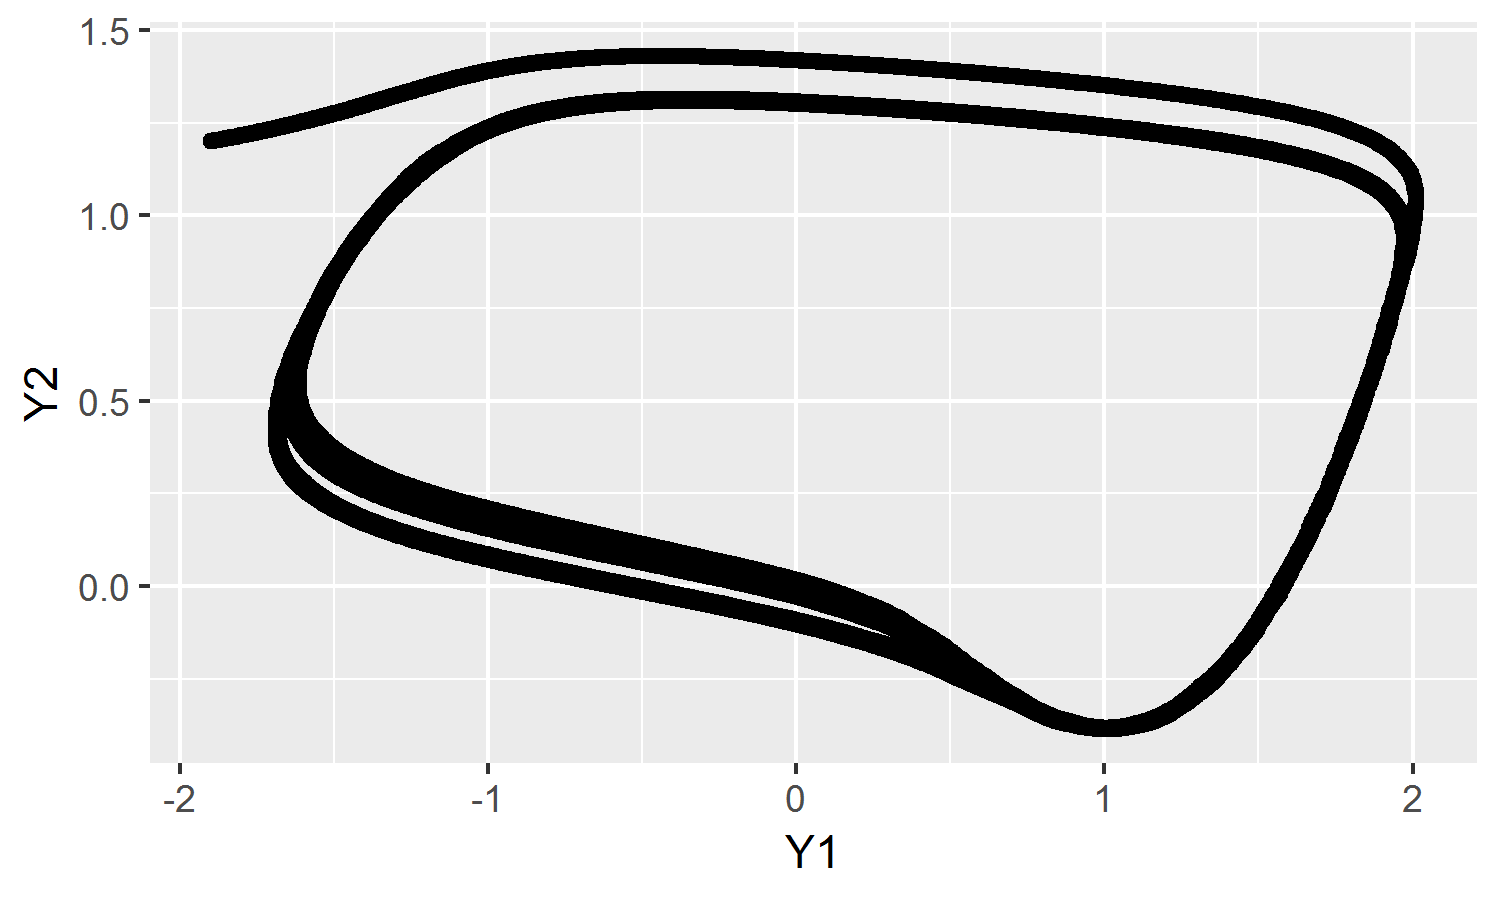
\includegraphics[width=\textwidth]{part1a-sigma2-Y1Y2.png}
        \caption{$\sigma = 0.20$}
    \end{subfigure}
    ~
    \begin{subfigure}[b]{0.45\textwidth}
        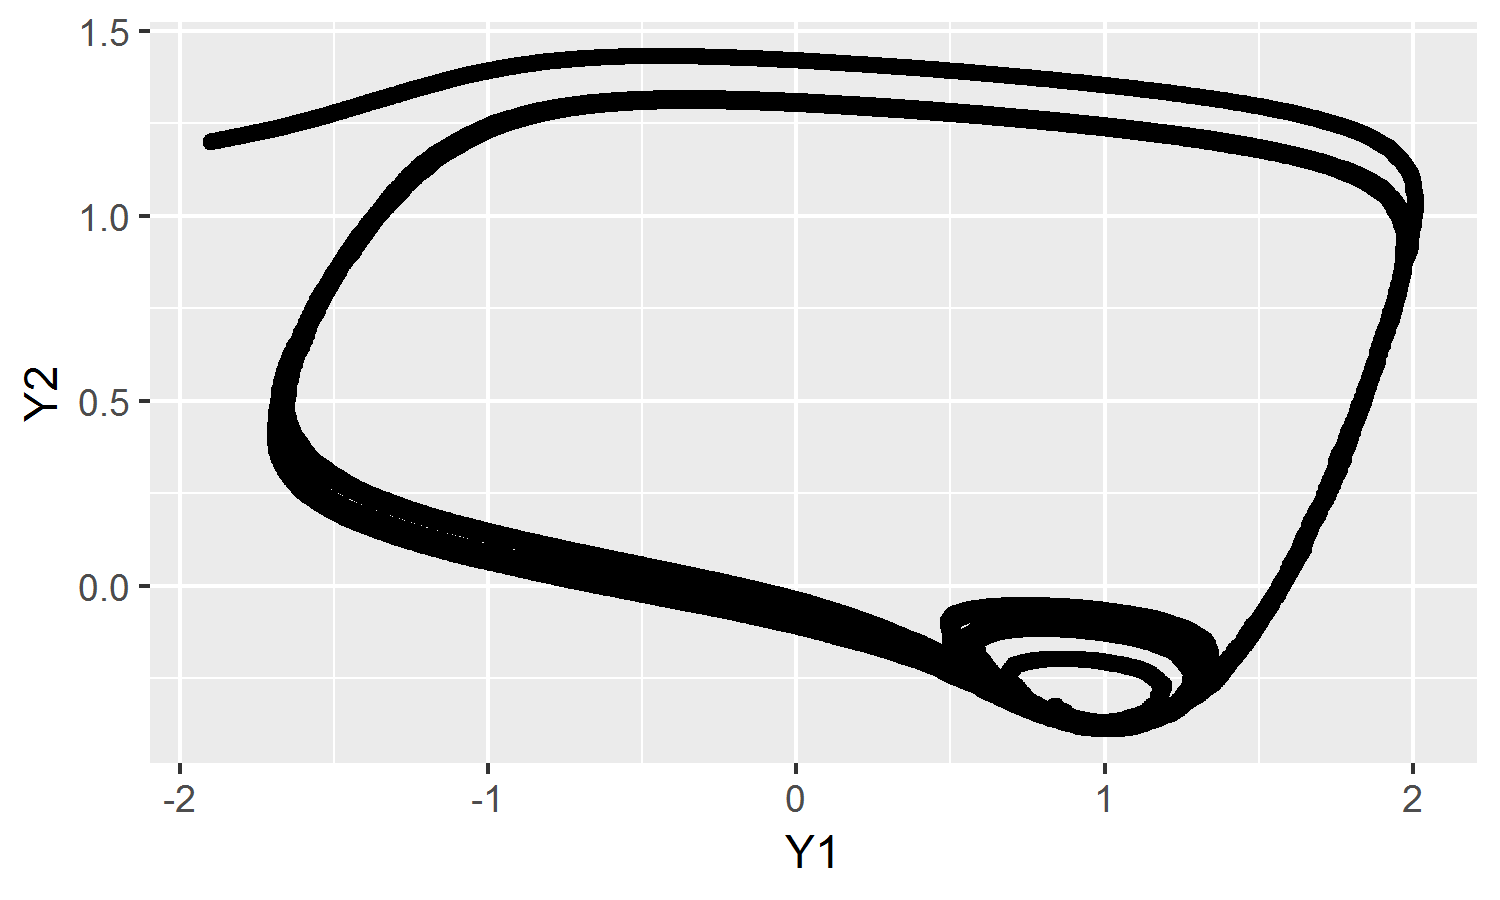
\includegraphics[width=\textwidth]{part1a-sigma3-Y1Y2.png}
        \caption{$\sigma = 0.30$}
    \end{subfigure}
    ~
    \begin{subfigure}[b]{0.45\textwidth}
        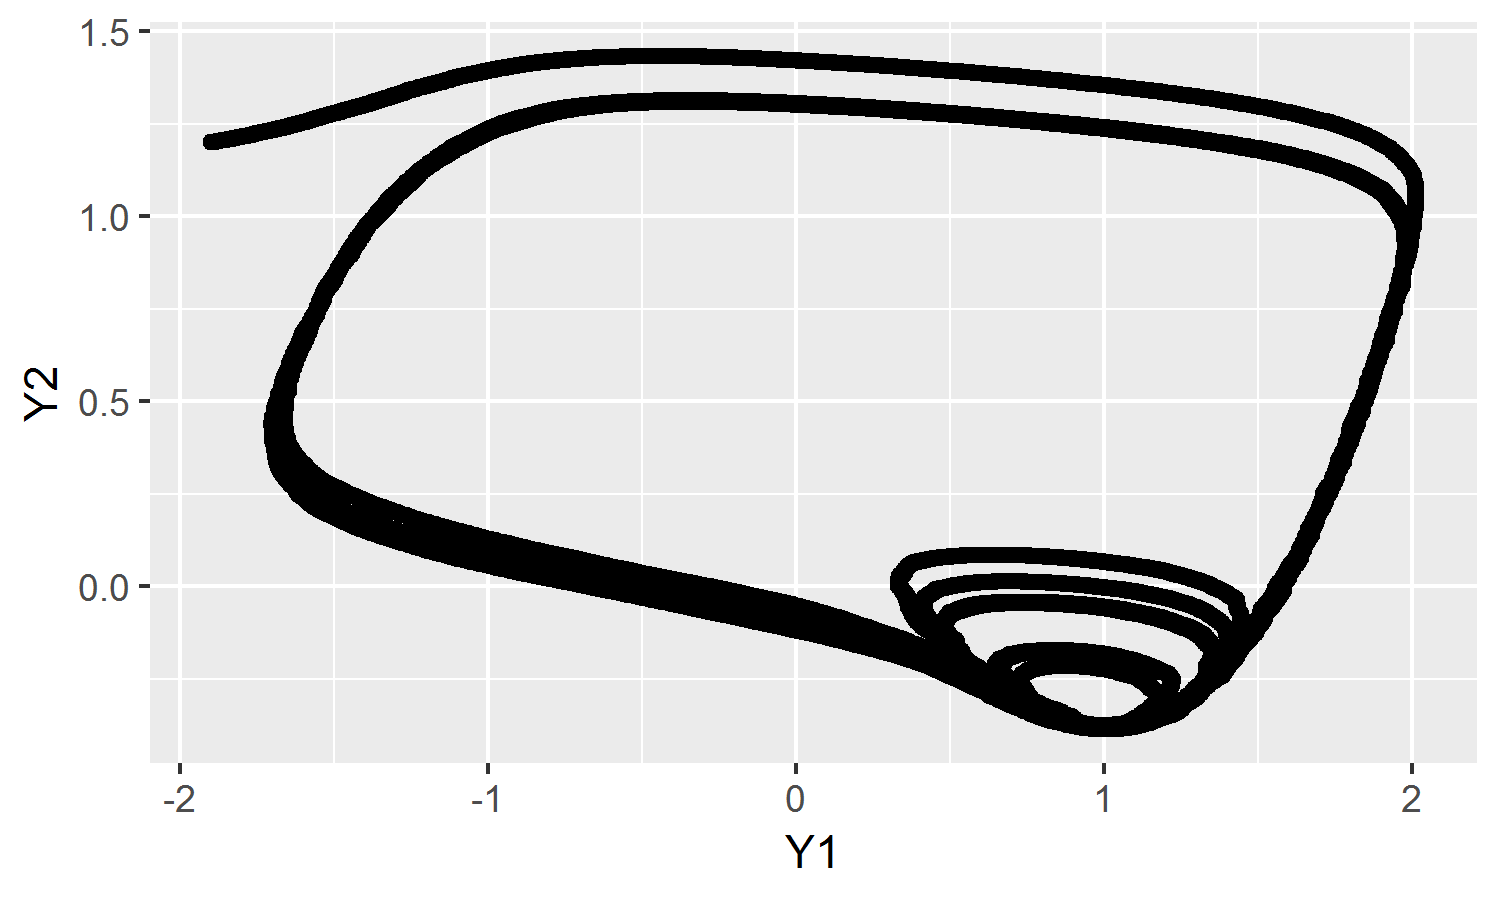
\includegraphics[width=\textwidth]{part1a-sigma4-Y1Y2.png}
        \caption{$\sigma = 0.40$}
    \end{subfigure}
    \caption{Phaseplots values of ($Y^1$, $Y^2$)}\label{fig:part1a-grid}
\end{figure}

\clearpage

\subsection{Question 1b}
Let $\sigma = 0.10$ and simulate using the approximation. Partition the phase plane in $100 \times 100$ equal cells. Count
the number of trajectories that passes through each cell. Repeat for $\sigma = 0.20, 0.30$ and $0.40$.

Which extra information does the plot contain, compared to the standard
phase-plot?

What we have plotted in \Cref{fig:part1b-grid} is count heatmap, and not
the number of time a trajectory passes through each cell. We think that 
the count heatmap is more informative, as it can reveal the speeds of the
trajectories at each cell. Higher counts could indicate slower moving passes of the cell.

\begin{figure}[ht!]
    \centering
    \begin{subfigure}[b]{0.45\textwidth}
        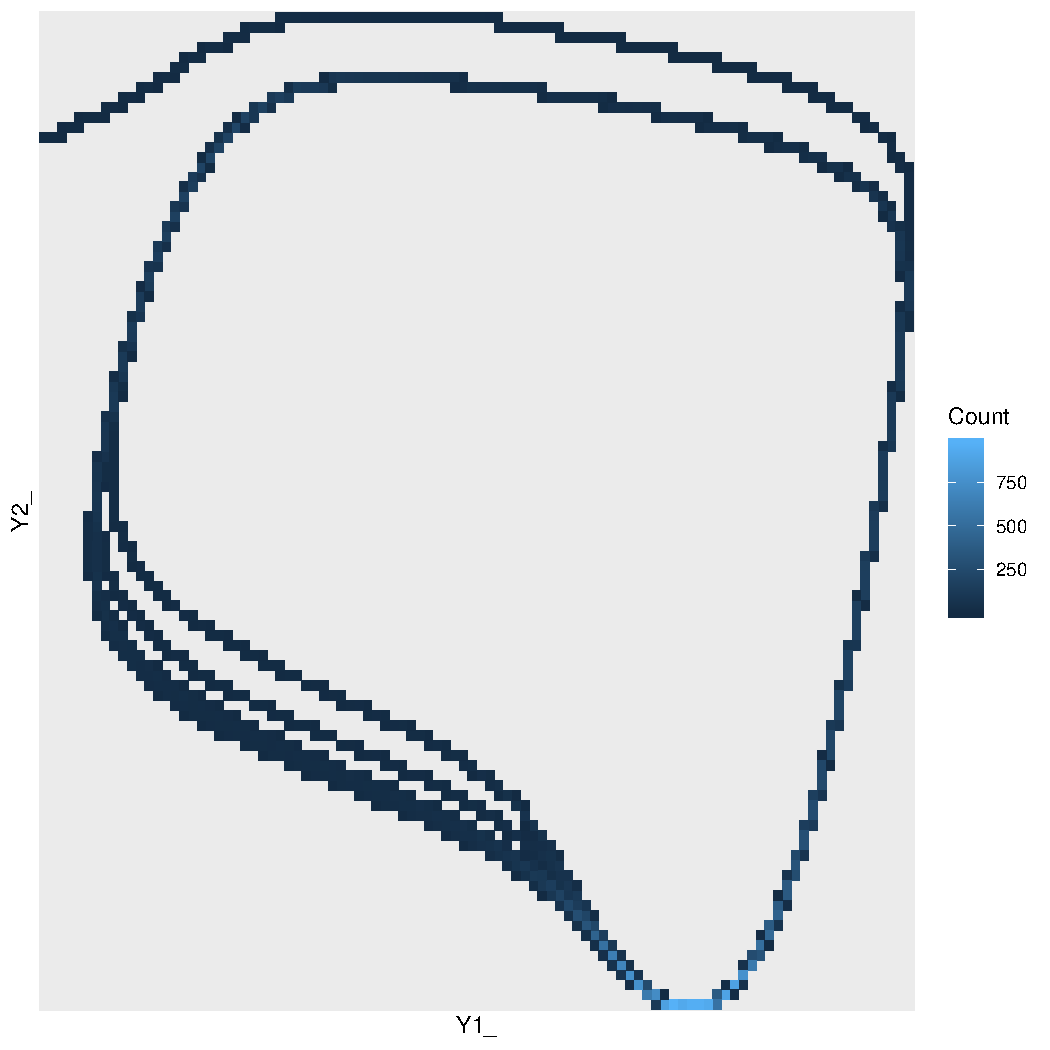
\includegraphics[width=\textwidth]{part1b-sigma1-grid.pdf}
        \caption{$\sigma = 0.10$}
    \end{subfigure}
    ~
    \begin{subfigure}[b]{0.45\textwidth}
        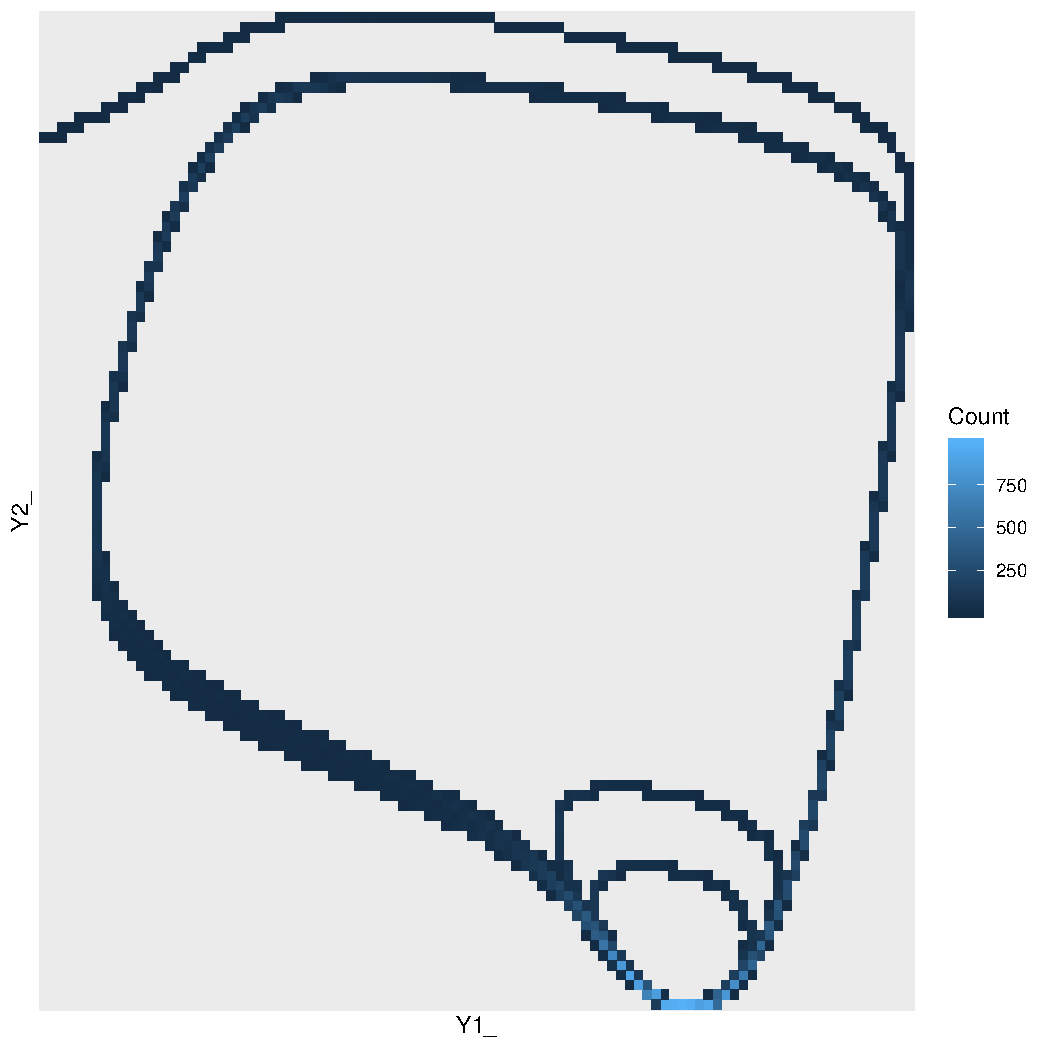
\includegraphics[width=\textwidth]{part1b-sigma2-grid.pdf}
        \caption{$\sigma = 0.20$}
    \end{subfigure}
    ~
    \begin{subfigure}[b]{0.45\textwidth}
        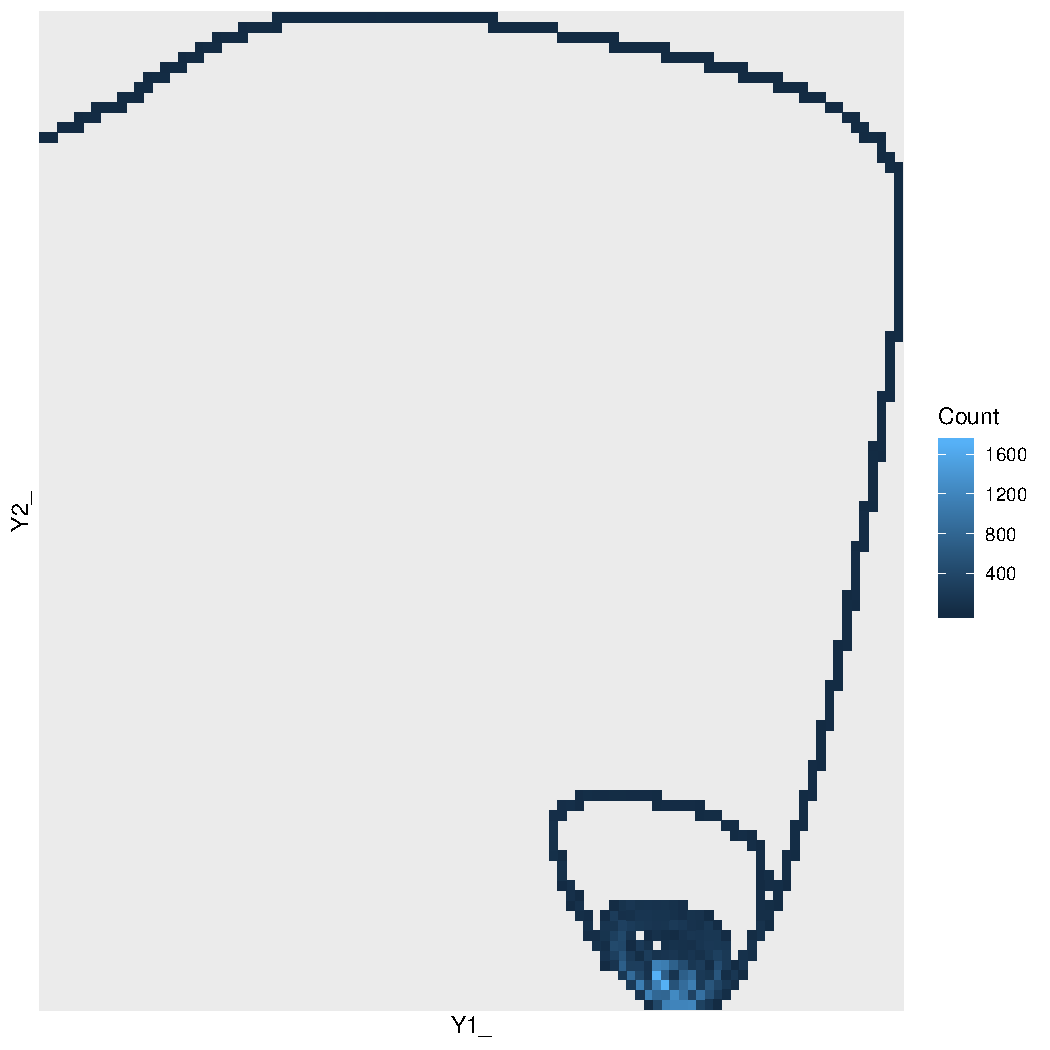
\includegraphics[width=\textwidth]{part1b-sigma3-grid.pdf}
        \caption{$\sigma = 0.30$}
    \end{subfigure}
    ~
    \begin{subfigure}[b]{0.45\textwidth}
        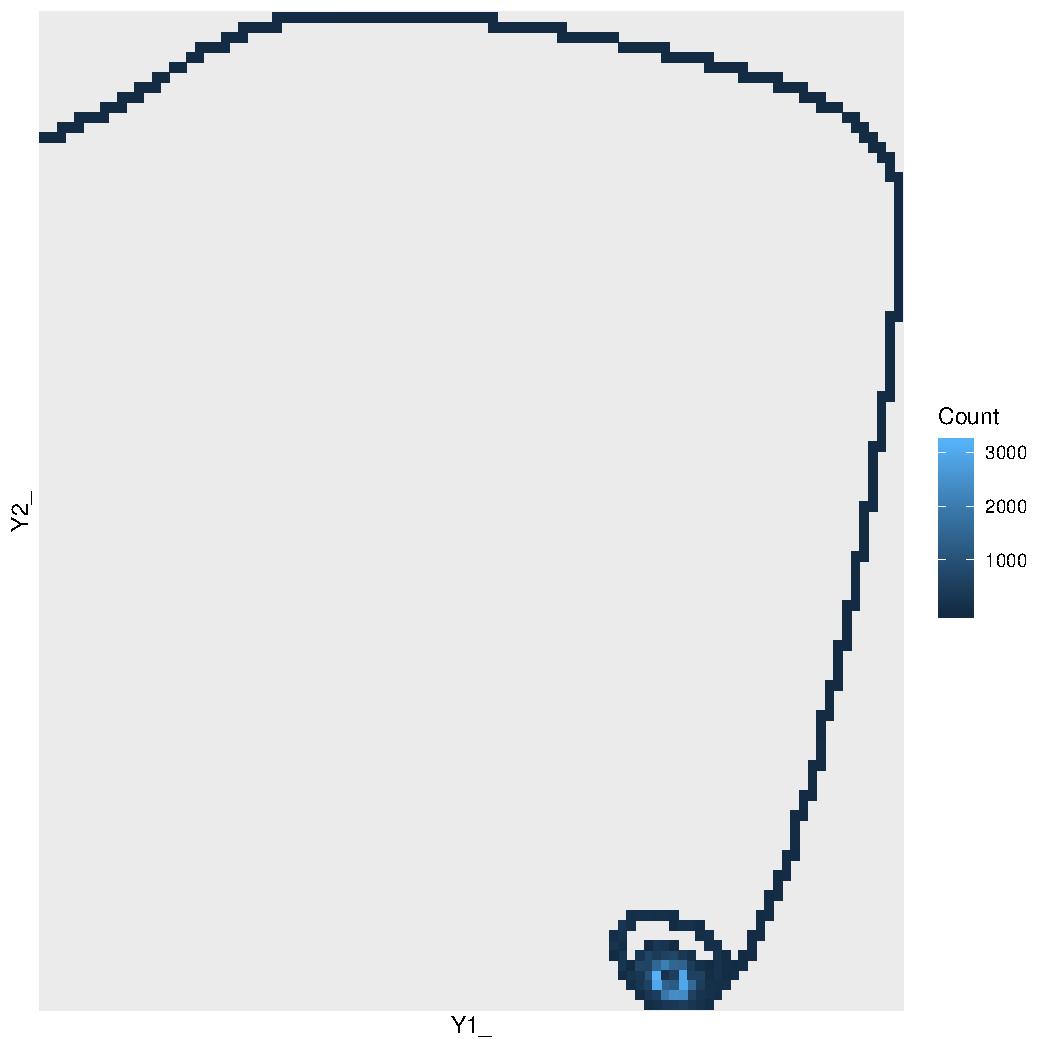
\includegraphics[width=\textwidth]{part1b-sigma4-grid.pdf}
        \caption{$\sigma = 0.40$}
    \end{subfigure}
    \caption{Realized values of $Y^1$ and $Y^2$ for $\sigma = 0.20$}\label{fig:part1b-grid}
\end{figure}
\clearpage

\section{Part 2}

We start our analysis with a exploration and some descriptive statistics of the source data. \Cref{fig:part2a-corr} shows correlations in the input data. We emphasize some insights:

\begin{enumerate}
    \item All four room temperatures, $yT_1, \ldots yT_4$, are quite strongly linearly correlated.
    \item The ambient temperature, $T_a$ seems to cause a lower bound on the room temperatures $yT_1, \ldots yT_4$. I.e.\ when it is hot outside, it will also be hot inside, which makes good sense, as there are no cooling units in the building.
    \item The solar radiation, $G_v$, seems to cause a lower bound on the ambient temperature. I.e. when the sun is shining strong, it will be warmer, which also makes good sense. With the above in mind, this also influences the inside temperatures.
    \item The heaters influence influences the inside temperature, $yT_1, \ldots yT_4$, but from this visualization, I argue, that it is not possible to see a difference. I.e. even though the northern circuit heater ($Ph_1$) is closer to room 1 and 2 ($yT_1, yT_2$), the correlation is almost the same as with the southern circuit heater $Ph_2$. 
\end{enumerate}

\begin{figure}[b!]
    \centering
    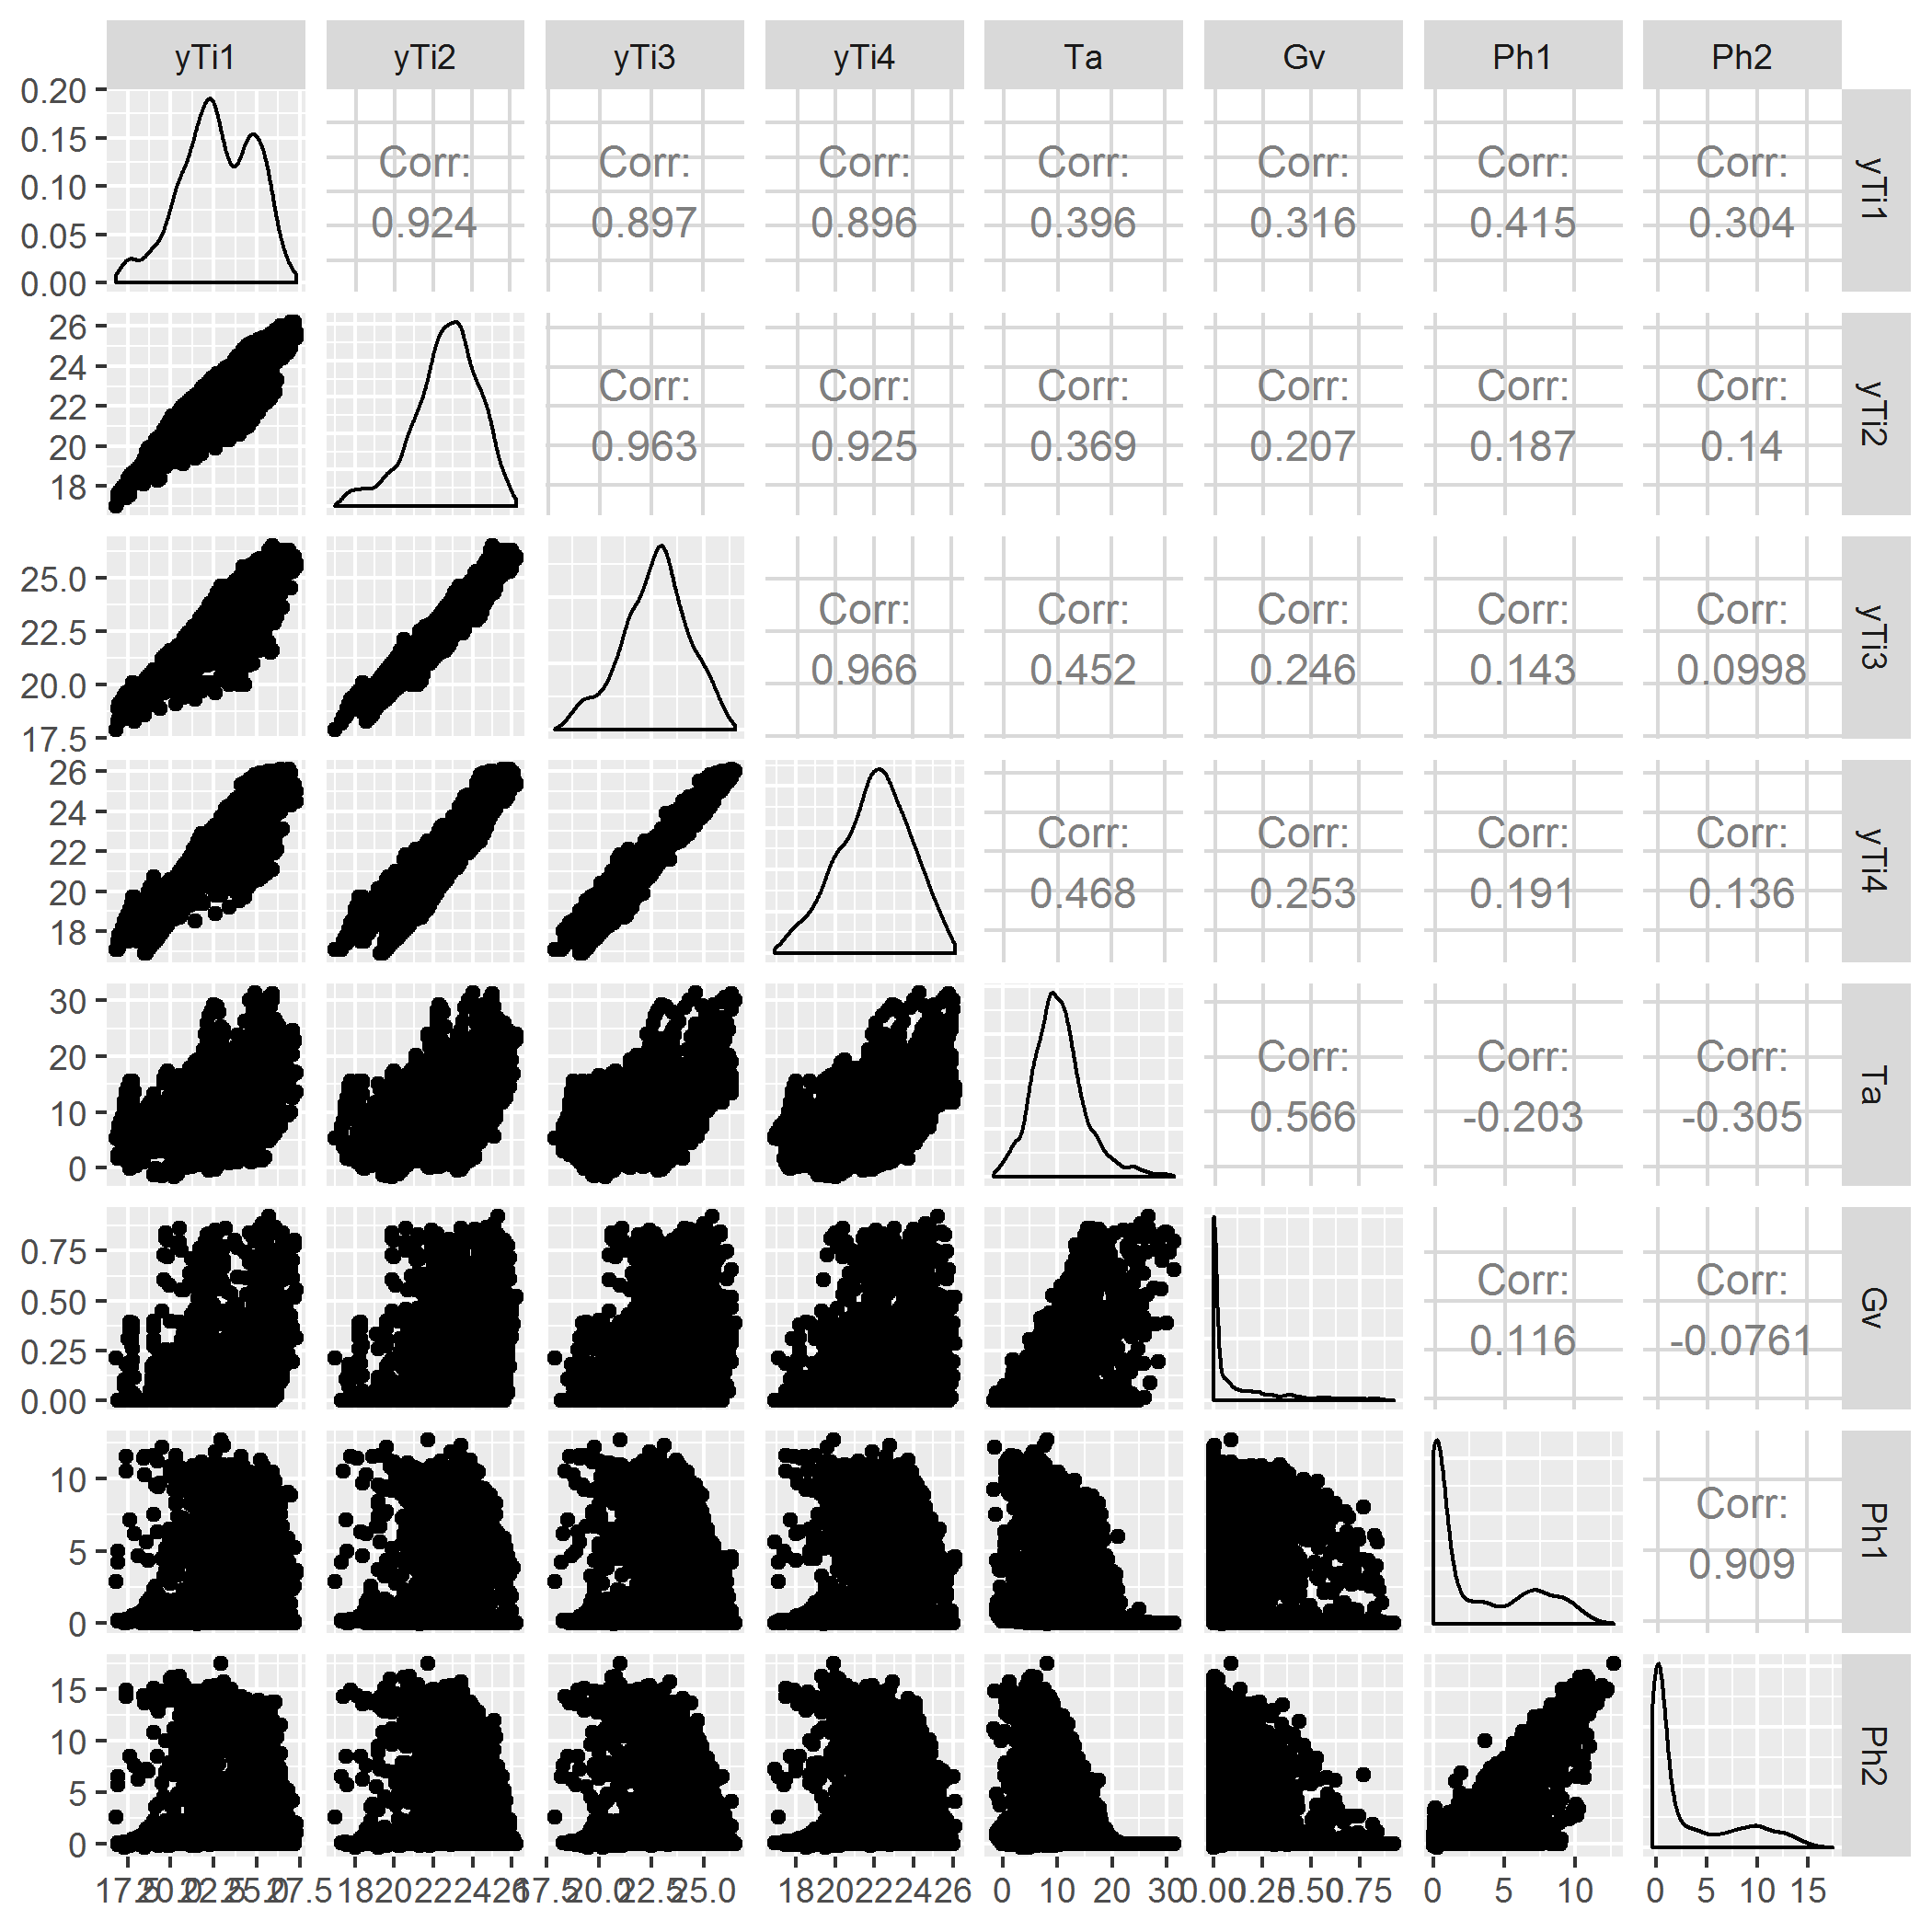
\includegraphics[width=.9\textwidth]{part2a-corr.png}
    \caption{Correlations in input data}
    \label{fig:part2a-corr}
\end{figure}
\clearpage

\subsection{Question 2a}
We modified the CTSM-R-model to include the 5 basis spline functions. For the initial guess for the 5 new parameters $a_1, \ldots, a_5$ we simply use $1$ and [$10^{-5}$; $10^{5}$] for the bounds.
\Cref{fig:part2a-fit-hour} shows the difference before and after the modification over the time of day. 
\Cref{tab:part2a} shows the improvement in MSE before and after the modification.

\begin{table}[ht!]
    \centering
    \begin{tabular}{cc}
        Model & MSE \\ \hline \hline
        Before modification  & 0.0852 \\ \hline
        After modification  & 0.0635 \\ \hline
    \end{tabular}
    \caption{Mean Squared Error (MSE) before and after modification.}
    \label{tab:part2a}
\end{table}

\begin{figure}[ht!]
    \centering
    \begin{subfigure}[b]{0.45\textwidth}
        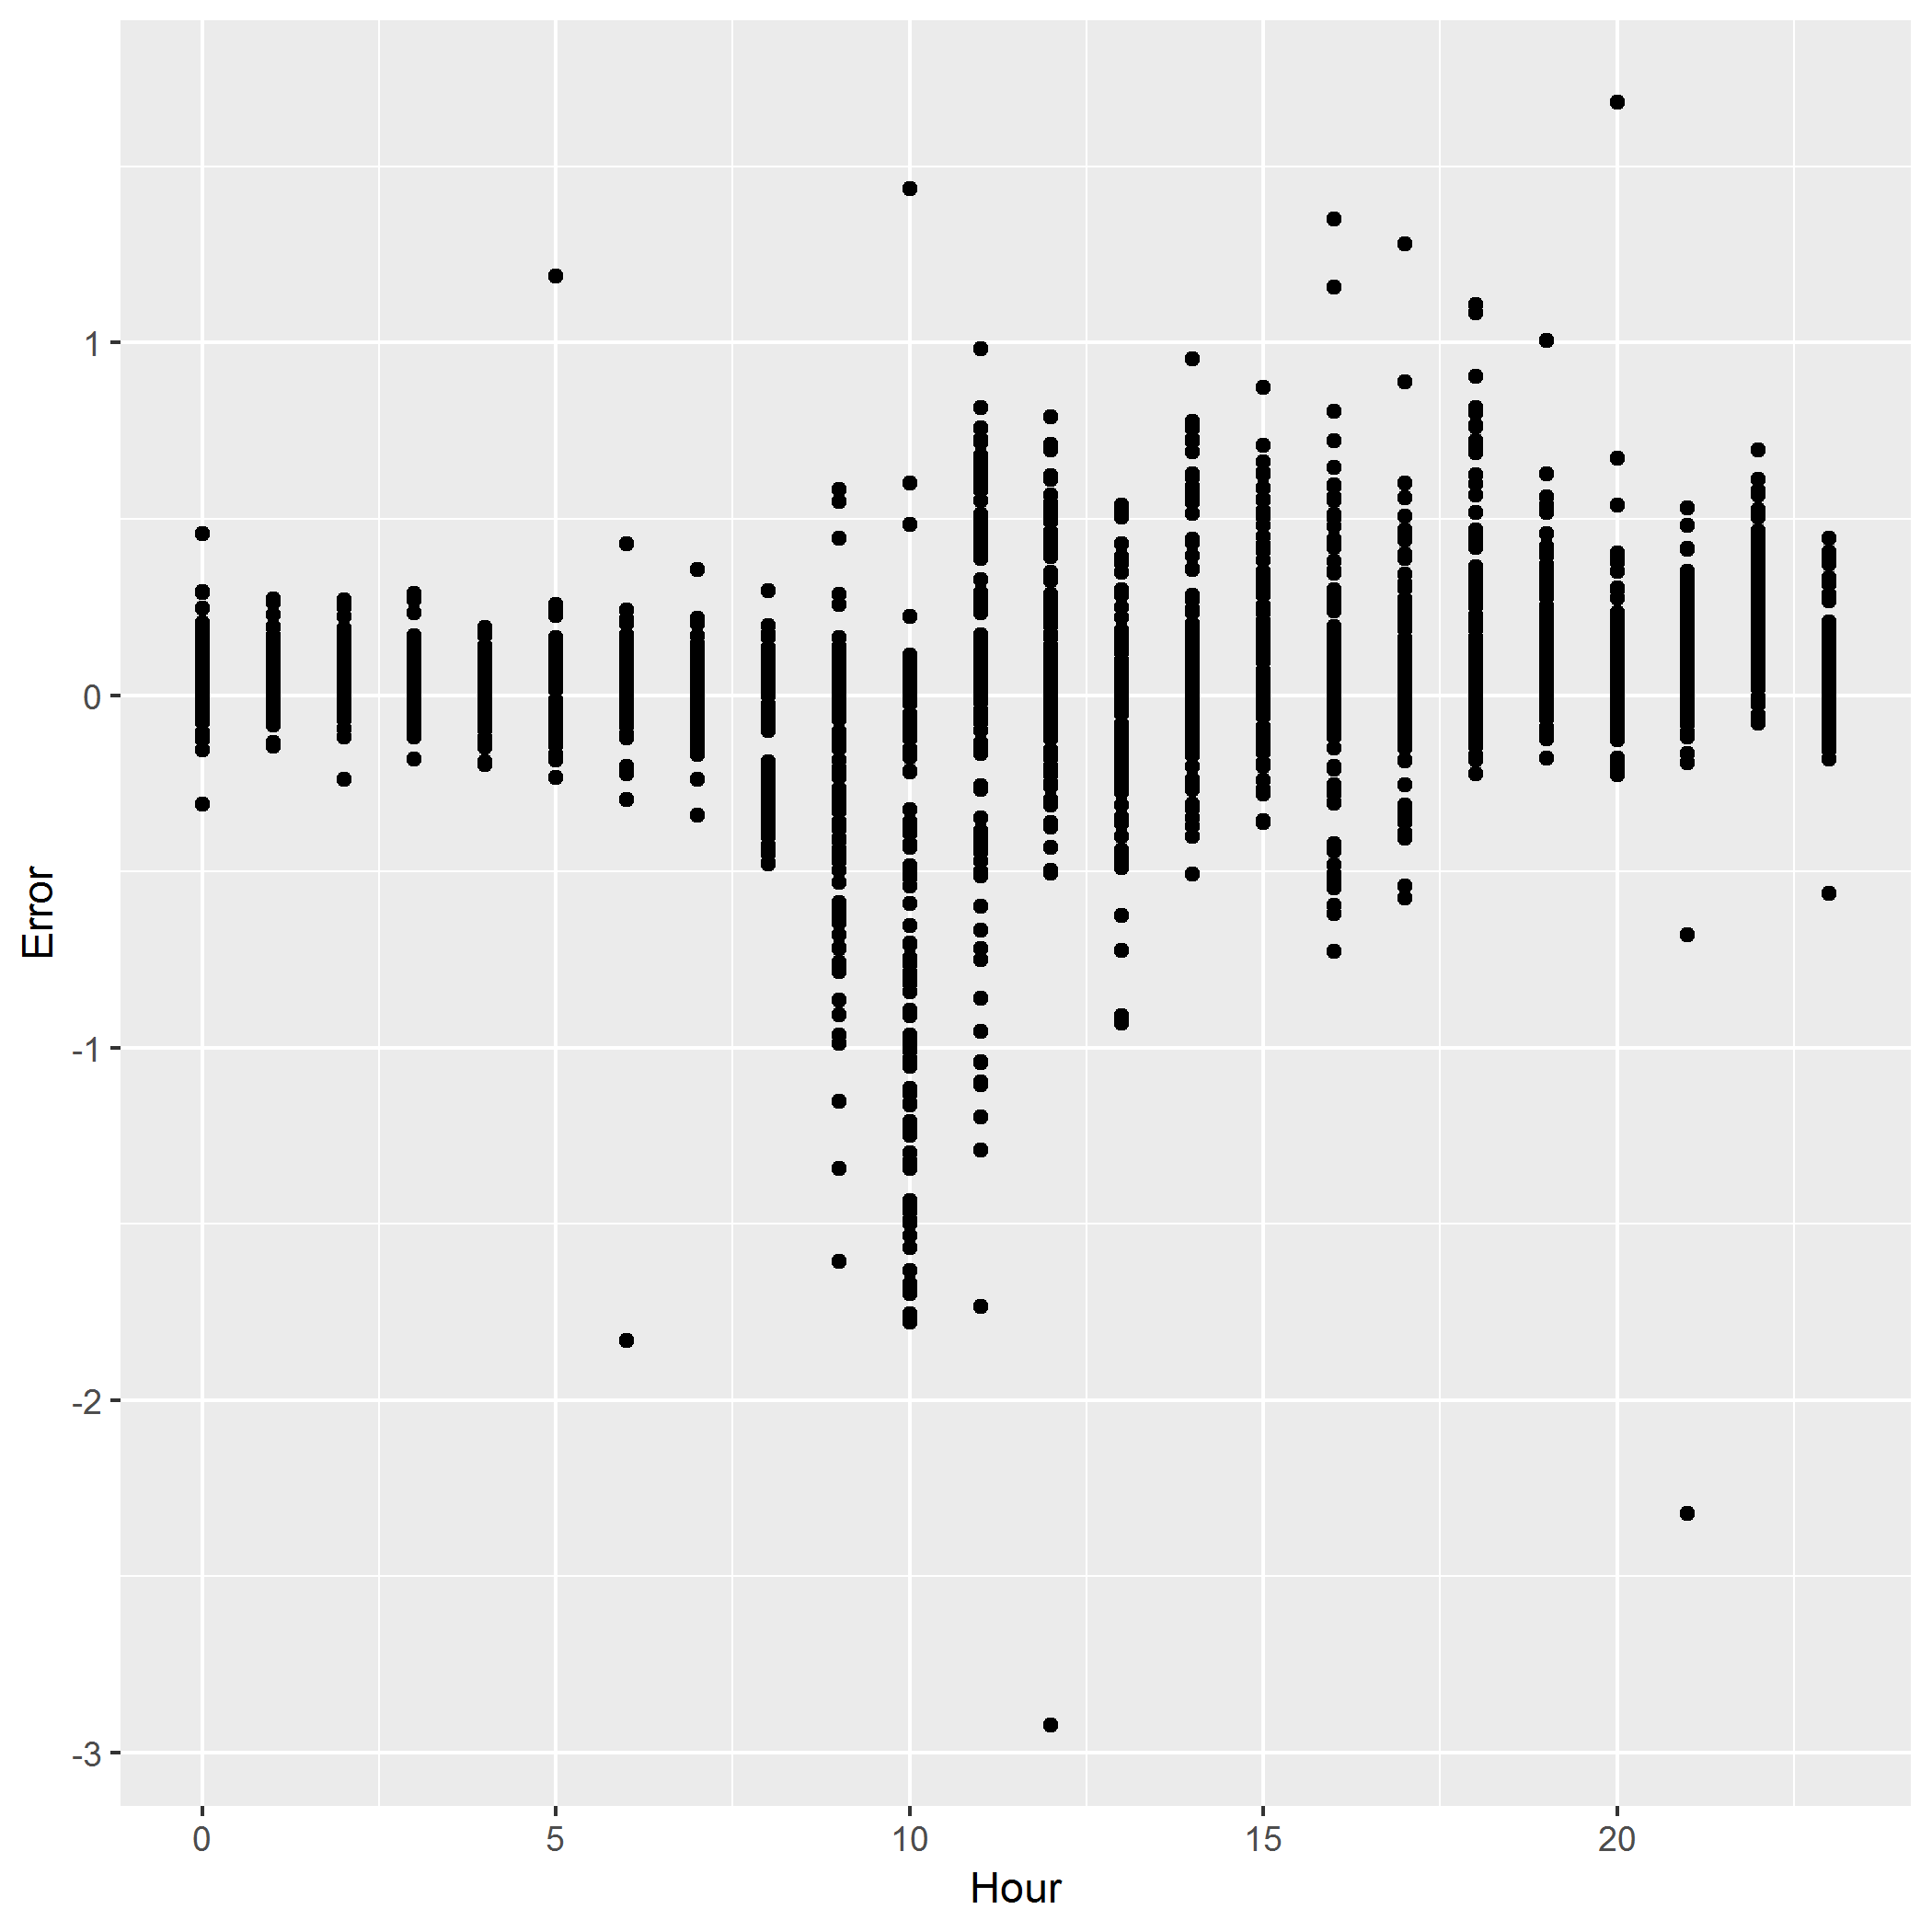
\includegraphics[width=\textwidth]{part2a-fit1-hour.png}
        \caption{Before modification}
    \end{subfigure}
    ~
    \begin{subfigure}[b]{0.45\textwidth}
        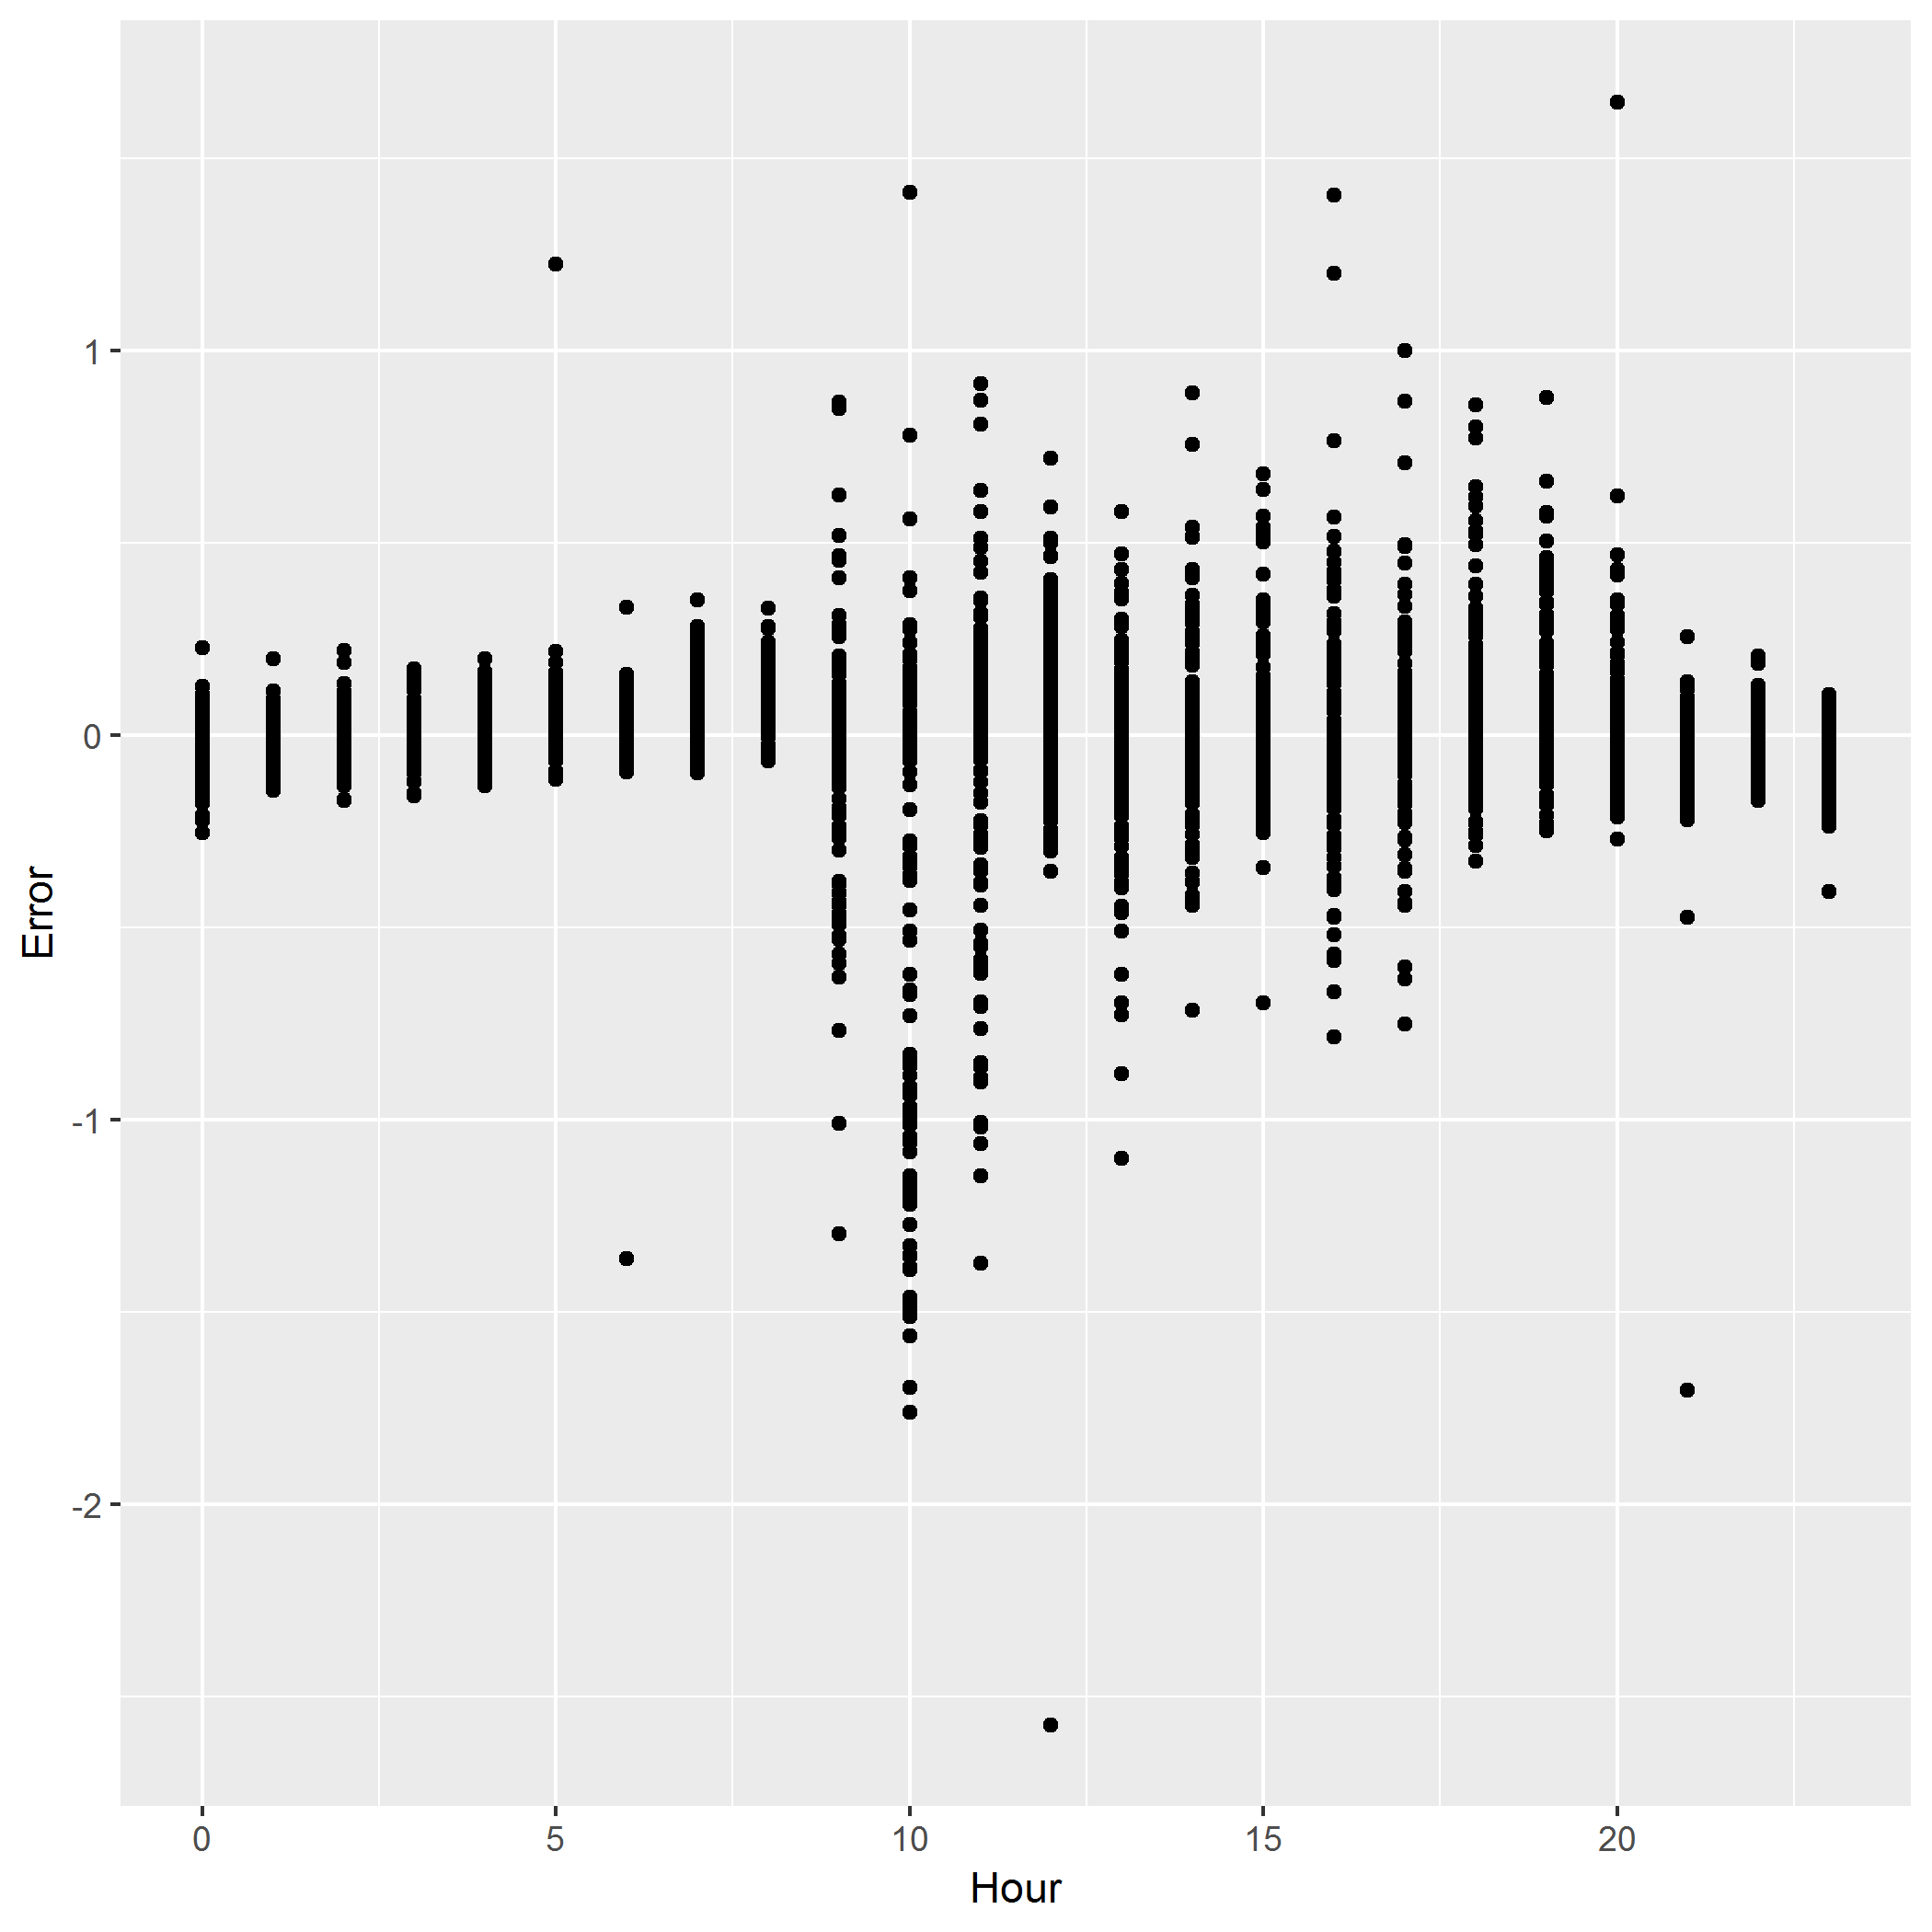
\includegraphics[width=\textwidth]{part2a-fit2-hour.png}
        \caption{After modification}
    \end{subfigure}
    \caption{Error over time of day before and after modification.}
    \label{fig:part2a-fit-hour}
\end{figure}

\subsection{Question 2b}
In this section, we explore some improvements to the model from 2a. Concrete we will consider the following two improvements:

\begin{enumerate}
    \item Incorporate heat transfer to/from nearby rooms. We think this could improve the model since the rooms share walls which surely can transfer heat.
    \item Incorporate heat transfer directly between thermal mass and the ambient air. This idea arowse since we are at the second floor, and a lot of the thermal mass of the building could be exposed to the ambient air.
\end{enumerate}

For the first improvement to be considered we have the following SDE-system:
\begin{align}
    dT_i &= {C_i}^{-1} \left( R_{ia}^{-1} (T_a - T_i) + R_{in}^{-1} (T_n - T_i) + R_{im}^{-1} (T_m - T_i) + \Phi + A(t) G_v \right) \mathit{dt} + \sigma_1 \mathit{dw}_1 \\
    dT_m &= {C_m}^{-1} \left( R_{im}^{-1} (T_i - T_m) \right) \mathit{dt} + \sigma_2 \mathit{dw}_2 
\end{align}

Where $A(t) = \sum_{k = 1}^{N} a_k \mathit{bs}_k(t)$, and $R_{in}$ is the thermal resistance between the current and nearby room, with temperature $T_n$. We run our expiriment on room $i = 1$ with the nearby room set to $n = 2$. After several tries we were unable to estimate parameters, even though we provided good initial guess for the new parameters (including $a_1, \ldots, a_k$). Further analysis showed that it is espacially the $A(t)$-term that causes the computational challange. We therefore chose to replace $A(t)$ with $Aw$ (as in the original model proposed in the excercise) and benchmark our improved model against the model \emph{before the modification} made in Section 2.1. 

The output of the parameter estimation is shown in \Cref{fig:improved_1}. We see the value of our new parameter $R_\mathit{in} = 25$ and is considered significant. This is also visible in the MSE for $T_i$ which is 0.0810 for our improved model compared to the original unmodified model with MAE for $T_i$  = 0.0852.

\begin{figure}[ht!]
\begin{lstlisting}[basicstyle=\footnotesize\ttfamily,frame=single,breaklines=true]
Coefficients:
          Estimate  Std. Error     t value    Pr(>|t|)     dF/dPar dPen/dPar
Ti10    2.3603e+01  1.8113e-01  1.3031e+02  0.0000e+00  4.1622e-02    0.0004
Tm0     1.0088e-11  1.0187e-10  9.9036e-02  9.2112e-01  0.0000e+00    0.0000
Aw      1.0621e-02  9.4214e-03  1.1274e+00  2.5967e-01  1.8185e-02   -0.0275
Ci      1.5823e+01  1.0765e+00  1.4698e+01  0.0000e+00  1.2370e+01    0.0000
Cm      1.2422e-01  1.5652e-02  7.9365e+00  2.8866e-15 -6.4670e-02    0.0000
e1     -1.2899e+01  2.0008e+01 -6.4469e-01  5.1918e-01 -3.2200e-02    0.0000
Ria     3.9138e+01  2.3833e+00  1.6422e+01  0.0000e+00  1.3814e+01    0.0000
Rim     4.1409e+01  7.9690e-03  5.1962e+03  0.0000e+00  1.4823e+00    0.0000
Rin     2.5025e+01  6.6420e-03  3.7677e+03  0.0000e+00  5.1819e+00    0.0000
sigma1 -1.7608e+00  2.4410e-02 -7.2135e+01  0.0000e+00 -4.0577e-02    0.0000
sigma2  4.8581e+00  1.0346e-01  4.6956e+01  0.0000e+00  1.5232e-01    0.0002

Correlation of coefficients:
        Ti10  Tm0   Aw    Ci    Cm    e1    Ria   Rim   Rin   sigma1
Tm0    -0.01
Aw     -0.02 -0.05
Ci     -0.05  0.36  0.03
Cm      0.04 -0.25 -0.02 -0.75
e1      0.00 -0.08  0.09 -0.07  0.02
Ria     0.05 -0.35 -0.05 -1.00  0.75  0.00
Rim    -0.05  0.36 -0.09  0.99 -0.76 -0.06 -0.99
Rin    -0.01 -0.02  0.11  0.04 -0.68  0.04 -0.05  0.04
sigma1  0.04 -0.05 -0.02 -0.26  0.45 -0.11  0.27 -0.26 -0.40
sigma2 -0.05  0.34  0.03  0.92 -0.89 -0.04 -0.92  0.92  0.33 -0.42
\end{lstlisting}
\caption{Parameter estimates for \emph{Improved Model 1}}
\label{fig:improved_1}
\end{figure}

For the second improvement we further modify the SDE to the following. I.e. we include a new parameter $R_{ma}$ for the heat transfer between the thermal mass and the ambient temperature.
\begin{align}
    dT_i &= {C_i}^{-1} \left( R_{ia}^{-1} (T_a - T_i) + R_{in}^{-1} (T_n - T_i) + R_{im}^{-1} (T_m - T_i) + \Phi + A(t) G_v \right) \mathit{dt} + \sigma_1 \mathit{dw}_1 \\
    dT_m &= {C_m}^{-1} \left( R_{im}^{-1} (T_i - T_m) + R_{ma}^{-1} (T_a - T_m)  \right) \mathit{dt} + \sigma_2 \mathit{dw}_2 
\end{align}

Unfortunately this does not improve the model, as the CTSM-algorithm terminales after only 6 iterations with MAE = $0.1305$.

\subsection{Question 2c}
In this section we present a multi-room model that describes
the heat dynamics of the 4 rooms that we got measurements from.

In order to simplefy the model we make some assumptions:
\begin{enumerate}
    \item The thermal resistance between the air and thermal mass is the same for all rooms, denoted $R_m$. This is assumed since all the rooms are on the same floor, and it seem likely that the floor is made of the same material in all the rooms. 
    \item The thermal resistance between the internal air and the outside is the same for room 1 and 4 ($R_o$), and room 2 and 3 ($R_h$). This is assumed since both room 1 and 2 are offices close to the outside, while room 2 and 3 seem like hallway and is more central in the building.
    \item The thermal capacity is the same for room 1 and 4 ($C_o$), and room 2 and 3 ($C_h$). This is assumed since both room 1 and 4 are offices of similar size, while room 2 and 3 seem like hallway and of larger, but similar size.
    \item We estimate the window area size for each room ($A_{w,1}, \ldots, A_{w,4}$) independently of the time, but allows for different window areas (and directions of the windows) for each window.
\end{enumerate}

\begin{align}
    dT_1 &= {C_o}^{-1} \left( R_o^{-1} (T_a - T_1) + R_m^{-1} (T_m - T_1) + \Phi_1 + A_{w,1} G_v \right) \mathit{dt} + \sigma_1 \mathit{dw}_1 \\
    dT_2 &= {C_h}^{-1} \left( R_h^{-1} (T_a - T_2) + R_m^{-1} (T_m - T_2) + \Phi_1 + A_{w,2} G_v \right) \mathit{dt} + \sigma_2 \mathit{dw}_2 \\
    dT_3 &= {C_h}^{-1} \left( R_h^{-1} (T_a - T_3) + R_m^{-1} (T_m - T_3) + \Phi_2 + A_{w,3} G_v \right) \mathit{dt} + \sigma_3 \mathit{dw}_3 \\
    dT_4 &= {C_o}^{-1} \left( R_o^{-1} (T_a - T_4) + R_m^{-1} (T_m - T_4) + \Phi_2 + A_{w,4} G_v \right) \mathit{dt} + \sigma_4 \mathit{dw}_4 \\
    dT_m &= {C_m}^{-1} \left( \sum_{i = 1}^4 R_m^{-1} (T_i - T_m) \right) \mathit{dt} + \sigma_5 \mathit{dw}_5 
\end{align}

Finally we present one last multi room model that takes into account the inter-room heat transfer we saw significant in the previous section. For this we introduce 3 new parameters to estimate: $R_{n,1,2}$, $R_{n,2,3}$, $R_{n,3,4}$. In this $R_{n,j,k}$ is the thermal resistance between room $j$ and $k$. The SDE for the system is shown in \cref{eq:mr2}. 

\begin{equation}
    \begin{aligned}
    dT_1 &= {C_o}^{-1} ( R_o^{-1} (T_a - T_1) \\
         &+ R_{n,1,2}^{-1} (T_2 - T_1) \\
         &+ R_m^{-1} (T_m - T_1) + \Phi_1 + A_{w,1} G_v ) \mathit{dt} + \sigma_1 \mathit{dw}_1 \\
    dT_2 &= {C_h}^{-1} ( R_h^{-1} (T_a - T_2) \\
         &+ R_{n,1,2}^{-1} (T_1 - T_2) + R_{n,2,3}^{-1} (T_3 - T_2) \\
         &+ R_m^{-1} (T_m - T_2) + \Phi_1 + A_{w,2} G_v ) \mathit{dt} + \sigma_2 \mathit{dw}_2 \\
    dT_3 &= {C_h}^{-1} ( R_h^{-1} (T_a - T_3) \\
        &+ R_{n,2,3}^{-1} (T_2 - T_3) + R_{n,3,4}^{-1} (T_4 - T_3) \\
        &+ R_m^{-1} (T_m - T_3) + \Phi_2 + A_{w,3} G_v ) \mathit{dt} + \sigma_3 \mathit{dw}_3 \\
    dT_4 &= {C_o}^{-1} ( R_o^{-1} (T_a - T_4) \\
        &+ R_{n,3,4}^{-1} (T_3 - T_4) \\
        &+ R_m^{-1} (T_m - T_4) + \Phi_2 + A_{w,4} G_v ) \mathit{dt} + \sigma_4 \mathit{dw}_4 \\
    dT_m &= {C_m}^{-1} \left( \sum_{i = 1}^4 R_m^{-1} (T_i - T_m) \right) \mathit{dt} + \sigma_5 \mathit{dw}_5 
    \end{aligned}
    \label{eq:mr2}
\end{equation}

This model takes quite some time to run on standard commodity hardware, but show slightly better overall performance as shown by the MSE results in \Cref{tab:part2c}. It is worth noticing that $T_1$ is actual a litle worse, while $T_2, \ldots, T_4$ is quite better, releatively speaking.

\begin{table}[ht!]
    \centering
    \begin{tabular}{ccc}
        Model / MSE & Multi room model 1 & Multi room model 2 \\ \hline \hline
        $T_1$  & 0.0836 & 0.1021 \\ \hline
        $T_2$  & 0.0304 & 0.0241 \\ \hline
        $T_3$  & 0.0373 & 0.0173 \\ \hline
        $T_4$  & 0.0373 & 0.0234 \\ \hline
        Mean   & 0.0472 & 0.0417
    \end{tabular}
    \caption{Mean Squared Error (MSE) for the multi room models.}
    \label{tab:part2c}
\end{table}

The full parameter estimation for \emph{Multi room model 2} is shown in \Cref{fig:part2c}. Again it is visible from the output, that the additional parameters, $R_{n,1,2}$, $R_{n,2,3}$, $R_{n,3,4}$, are significant.

\begin{figure}
\begin{lstlisting}[basicstyle=\footnotesize\ttfamily,frame=single,breaklines=true]
Coefficients:
        Estimate  Std. Error    t value  Pr(>|t|)
T10     2.3584e+01  2.4516e-01    96.1986 < 2.2e-16 ***
T20     2.2234e+01  1.1898e-01   186.8673 < 2.2e-16 ***
T30     2.2771e+01  9.4945e-02   239.8396 < 2.2e-16 ***
T40     2.2005e+01  8.7128e-02   252.5609 < 2.2e-16 ***
Tm0     1.8840e-02  4.3778e-03     4.3035 1.695e-05 ***
Aw1     6.7601e+00  1.0759e+00     6.2832 3.442e-10 ***
Aw2     3.8781e+00  8.5857e-01     4.5169 6.339e-06 ***
Aw3     8.2243e+00  7.7850e-01    10.5643 < 2.2e-16 ***
Aw4     8.2784e+00  7.3707e-01    11.2315 < 2.2e-16 ***
Ch      5.1066e+01  9.6463e-01    52.9383 < 2.2e-16 ***
Cm      5.1049e-02  2.9864e-03    17.0940 < 2.2e-16 ***
Co      3.7258e+01  7.3398e-01    50.7619 < 2.2e-16 ***
e1     -4.9983e+00  1.9962e-03 -2503.8741 < 2.2e-16 ***
e2     -4.9989e+00  6.1805e-04 -8088.2422 < 2.2e-16 ***
e3     -4.9990e+00  9.7036e-04 -5151.6560 < 2.2e-16 ***
e4     -4.9989e+00  6.5796e-04 -7597.6671 < 2.2e-16 ***
Rh      2.8874e+00  4.4598e-02    64.7433 < 2.2e-16 ***
Rm      1.9949e+02  2.9903e+00    66.7127 < 2.2e-16 ***
Rn12    1.0531e+00  4.0271e-02    26.1515 < 2.2e-16 ***
Rn23    4.1390e+01  2.8227e-01   146.6301 < 2.2e-16 ***
Rn34    8.8741e+00  1.0321e-01    85.9849 < 2.2e-16 ***
Ro      2.6021e+00  4.8616e-02    53.5234 < 2.2e-16 ***
sigma1 -1.5331e+00  1.5072e-02  -101.7157 < 2.2e-16 ***
sigma2 -2.5629e+00  2.5395e-02  -100.9209 < 2.2e-16 ***
sigma3 -3.2397e+00  5.9319e-02   -54.6156 < 2.2e-16 ***
sigma4 -2.4894e+00  2.5982e-02   -95.8112 < 2.2e-16 ***
sigma5  6.7289e+00  3.2759e-02   205.4069 < 2.2e-16 ***
---
Signif. codes:  0 '***' 0.001 '**' 0.01 '*' 0.05 '.' 0.1 ' ' 1
\end{lstlisting}
\caption{Parameter estimates for \emph{Multi room model 2}}
\label{fig:part2c}
\end{figure}

\end{document}
